\documentclass[openright]{report}
\usepackage[utf8]{inputenc}
\usepackage[table]{xcolor}
\usepackage{fancyhdr}
\usepackage{extramarks}
\usepackage{amsmath}
\usepackage{amssymb}
\usepackage{flafter} 
\usepackage{amsthm}
\usepackage{multicol}
\usepackage{amsfonts}
\usepackage{tikz}
\usepackage[plain]{algorithm}
\usepackage{forest}
\usepackage{algpseudocode}
\usepackage{changepage}
\usepackage{siunitx}
\usepackage{wasysym}
\usepackage{mathtools}
\usepackage{titlesec}
\usepackage{indentfirst}
\usepackage{graphicx}
\usepackage{titletoc}
\usepackage{array}
\usepackage[toc,page]{appendix}
\usepackage[hyphens,spaces,obeyspaces]{url}
\usepackage{tabulary}
\usepackage[labelformat=empty]{caption}
\usepackage[english]{babel}
\usepackage[nottoc]{tocbibind}
\usepackage{chngcntr}
\counterwithout{figure}{chapter}
\usepackage[T1]{fontenc}
\usepackage{listings}
\usepackage{xcolor}
\usepackage[scaled=.85]{beramono}

\newcolumntype{K}[1]{>{\centering\arraybackslash}p{#1}}

\graphicspath{ {images/} }
\usetikzlibrary{automata,positioning}

\usetikzlibrary{shapes.geometric, arrows}

\tikzstyle{startstop} = [rectangle, rounded corners, minimum width=3cm, minimum height=1cm,text centered, draw=black, fill=red!30]
\tikzstyle{io} = [trapezium, trapezium left angle=70, trapezium right angle=110, minimum width=3cm, minimum height=1cm, text centered, draw=black, fill=blue!30]
\tikzstyle{process} = [rectangle, minimum width=3cm, minimum height=1cm, text centered, text width=3cm, draw=black, fill=orange!30]
\tikzstyle{decision} = [diamond, minimum width=3cm, minimum height=1cm, text centered, draw=black, fill=green!30]
\tikzstyle{arrow} = [thick,->,>=stealth]

\renewcommand{\familydefault}{\rmdefault}

\topmargin=-0.45in
\evensidemargin=0in
\oddsidemargin=0in
\textwidth=6.5in
\textheight=9.0in

\linespread{1.25}

\pagestyle{fancy}

\renewcommand{\chaptermark}[1]{\markboth{#1}{}}

\lhead{\projectAuthorShort}
\chead{\reportTopic}
\rhead{\leftmark}
\lfoot{\lastxmark}
\cfoot{\thepage}

\newcommand{\reportTopic}{Phase IV Report}
\newcommand{\projectAuthorShort}{Cybersecurity Education Group}
\newcommand{\projectTitle}{Project BrightSun}
\newcommand{\reportDueDate}{April 27, 2018}
\newcommand{\reportClass}{Synthesis Design II}
\newcommand{\reportClassInstructor}{Professor Dana Elzey}
\newcommand{\reportAuthorName}{Clark Benham (cb5ye), Calvin Krist (czk4ja), Saeed Razavi (slr4gf),\\and Jake Smith (jts5np)}
\newcommand{\collaborators}{}

\title{
    \vspace{2in}
    \LARGE{\textbf{\projectTitle}}\\
    \vspace{0.1in}\large{\reportClass:\ \reportTopic}\\
    \vspace{0.1in}\large{\reportClassInstructor}\\
    \normalsize\vspace{0.1in}\large{Due\ on\ \reportDueDate\ at 5:00pm}
    \vspace{1.4in}
}

\author{\reportAuthorName}
\date{}

\renewcommand{\contentsname}{Table of Contents}
\titlespacing*{\chapter}{0pt}{-40pt}{40pt}

\titleformat{\chapter}
  {\Large\bfseries} % format
  {}                % label
  {0pt}             % sep
  {\huge \vspace{-0.2in}}           % before-code

\begin{document}

\maketitle

\large{\tableofcontents}

\chapter{Introduction}

\par Software is ubiquitous across the world today. Companies use software to manage user data and offer services. Consumers use it to work, relax, and learn about the world. It's used by governments to help manage elections, recognize citizen needs, and protect their sovereignty. 

\par Software is also used for malicious purposes: criminals, both organized and free-lance, use software, called `malware', to attack businesses, consumers, and governments for personal gain. Malware is also used by activists such as Anonymous to damage those they view as harmful, such as their attack against the World Trade Organization \cite{anonymous_attack}. Even governments use malware for unethical purposes: the NSA's PRISM program was discovered to be conducting warrantless surveillance on U.S. citizens \cite{nsa_illegal}. High quality programs that costs millions to produce have been used to destroy infrastructure and attack nation states, such as Stuxnet, believed to have been made by the United States \cite{stuxnet}. Autocratic regimes, such as that in Lebanon, have used malware to spy on their own people and attack political dissidents \cite{lebanon}.

\par In order to combat malicious software, a specialized security field called `cybersecurity' arose that protects software systems and responds to attacks through a variety of means. Cybersecurity professionals from Gartner, an IT research company, defined the term as "security practices related to the combination of offensive and defensive actions involving or relying upon information technology and/or operational technology environments and systems" \cite{cyber_def}. In other words, the field of cybersecurity encompasses both attacking and defending systems such as computers, networks, and databases. Due to the components of these systems, cybersecurity professionals are often also called IT security professionals. This field is taught at many universities today, and cybersecurity professionals are in high demand from both companies and governments due to the pervasive integration of software into modern society, the high value of user data, and a lack of qualified professionals.

\section{Context and Environment}

\par Before diving into specifics regarding our solution, we first examine the context and environment in which our solution will operate.

\par In an economic context, there is currently a very competitive market for educational and technology based software. This competition continues to drive down prices and raise the overall quality of solutions available to the public. Additionally, with the rise of the open source development mentality of the general community, more and more training resources are being created, completely free for anyone to use and modify \cite{open_source}. By making these tools available under the MIT License or similar terms, creators are able to get more people using their tools. This higher adoption rate ultimately helps the creators better achieve their goal: creating a useful tool that adds value for someone in someway.

\par In continuing with this idea, we have elected to keep our project open-source and available to the public (ie free to use). By opening our project up to more people, we aim for two main benefits. First, with more active users of our product, more diverse and extensive feedback will be generated as we look to get our product in the hands of actual users. We can then in turn utilize this feedback to enhance our tool over time so that it is tailored to even more peoples' needs. In addition, one of our overarching goals for the project was to, in general, improve cybersecurity education for beginners. Therefore, it follows that with more people using our solution, our impact on the problem area will multiply. By adding any sort of fee to use our product, at least at this point, we think it would be cost prohibitive for our intended userbase.

\par In a socio-cultural context, as we have mentioned before, cybersecurity is a very recent and quickly evolving field. As a result, our solution will need to be modular enough that it can be easily adapted in the future. Our target audience for the project, students and professors, will remain the same throughout the lifespan of the project. As the years pass, new generations of students will be able to use the tool, so it is important that it can and will be updated regularly. In addition, as new software and operating systems are released, we will want to be able to integrate those into our solution easily. Another key aspect to recognize is that there will be a large influx of new students jumping into cybersecurity. With all of the major headlines about data breaches, hacks, and job openings, more people will be interested in participating in the field. As with the enrollment growth of computer science majors, we expect a similar double digit or better growth rate in cybersecurity focused students. Finally, in order for any tool to gain widespread popularity in today's world, the user experience is crucial. As such, we will need to ensure we are developing a product that provides ample instruction and an intuitive interface to help the users, especially beginners, as they use the product.

\par In a technological context, the technology needed to simulate complex business environments is finally reaching the real world. In following with Moore's Law, the computers of today are several times more powerful than those of just a few years ago. As a consequence of this, the required hardware for extensive virtualization is reaching mainstream adoption. As we continue to lower the barrier of entry in terms of capital, more and more students will be able to utilize tools such as ours to learn complex cybersecurity topics. From a software point of view, the concept of containerization has also become popular in recent years. With containerization, people, independent of a specific operating system, can run specific software \cite{docker}. This trend, along with virtualization, will enable us to build on the technologies others have to created to allow anyone on any platform to use our tool. With this portability, we expect that it will be easier for more widespread adoption of our solution. For example, if the professor does not need to worry as much about the details of all the students' machines, they can spend more time on creating the actual content for the lesson.

\section{Problem Overview}

\par Why are there so few cybersecurity job applicants and why are so few of them qualified? To begin, this is a very new field. As a result, there is no consensus as to what students should be taught and how they should be taught \cite{why_no_cyber_classes}. This means that there can be a large discrepancy between what employers want, what employers need, and what students are taught. Furthermore, not many universities offer undergraduate degrees in cybersecurity, much less a quality education in the field. This includes the University of Virginia. Here at UVA, there is currently a lot of debate between CS professors as to how much security education should be required to get a degree \cite{ibrahiminterview}. Currently, while numerous security courses are offered and more are coming, there is no requirement to take one \cite{comsci_handbook}. Students only study cybersecurity if it interests them.

\par This results in two things: normal software developers leave more vulnerabilities in their applications, and fewer students become interested in cybersecurity. Not teaching basic security to CS undergraduates means that those students, now professional developers, are not aware of the security needs of applications or the ways that they can expose user data. This means lots of software, much of which is used by consumers, have vulnerabilities that can be abused by malicious hackers \cite{why_no_cyber_classes}. If graduates were required to take basic security courses, they may be more cognizant of the security of their applications and consumers would be safer.

\par Furthermore, many students will not take cybersecurity courses unless it is required. Cybersecurity, in contrast to most of computer science, is very intimidating. It has a dry reputation, and it's generous to say that there are even \textit{basics} to cybersecurity, due to the high level of technical knowledge demanded to even begin to make progress. This disincentives those who might otherwise take the class to explore the field, and As we have seen by talking with students, many don't know where to begin studying the topic if they might instead chose to self-teach. 

\par Cybersecurity requires vast domain experience due to the diversity of systems that need to be protected. As a result, it's hard to learn and hard to become passionate about because there is no immediate payoff to studying it, in terms of skills acquired. Compare this with other introductory courses which at least allow one to solve, simplified, real world problems. This means that few students will become interested in the field on their own, and without universities pushing students towards towards the field, this problem will not be rectified.

\par Even for those who decide cybersecurity is a topic worth pursuing, there are many barriers. Much of cybersecurity is about the interaction of systems. This means that to do more than read about topics--to get hands on experience--students need to be able to set up or simulate the systems they read about. Students need to know more than just intermediate programming and network theory: they also need to be server experts, OS experts, and knowledgeable about service architecture. It is the connection between systems that is the most prone to security failures, as there is not always a unified system for examining interactions. This is shown by the Cisco 2017 Security Capabilities Benchmark Study, a survey of 400,000 members of the Information Security Community on Linked-In, which found at within the largest area of concern(cloud platforms at 90\%)the biggest threat is the misconfiguration of cloud platforms (62 percent ) \cite{Cisco}.

\par This asks a lot of students. The necessary complexity of these systems makes them difficult to set up, and even following an online tutorial is frustrating. Small differences in computer configurations can result in hours of hard work debugging the problem. This is very discouraging, and can slow down student learning or even dissuade them from the field entirely. 

\par These same problems are why many university graduates lack hands on experience and are unqualified for most IT security jobs. Because of the nature of teaching in a classroom, the labs have to work for all students. If the lab doesn't work on one student's computer, the professor is faced with a painful decision: to leave the student behind, or hold up the whole class to try and debug the issue. As a result, most labs are as simple as possible while still demonstrating core concepts to reduce the time spent setting up and the risk of a student not being able to participate \cite{ibrahiminterview}. This means that, for universities to give students hands on experience, the best technology right now is to have dedicated computer labs set up for students to use. This means a computer for every student - enough routers, servers, and equipment for all of them. This is incredibly expensive, take lots of time to set up, test, and prepare, and it still could fail.

\par The result is that schools can't give students hands on experience and students have lots of trouble getting that experience themselves. Thus, most of those that do choose to study this field lack the requisite experience necessary to be a qualified IT security professional.

\par In summary in order to combat these problems, our goal is to enable students to easily create systems that allow them to study cybersecurity. Our hope is that students, teachers, and professionals can use our product to make the field more approachable and increase the number and proficiency of cybersecurity professionals. This could make a dent on the lack of qualified IT security specialists, lessening the risks associated with a world becoming more and more digital.

\section{Customers and Target Audience}

\par Throughout this project, we actively consulted with 3 groups of people acting as the customers for our project. During our Sprint Reviews, we met with our customers to present the current solution, get feedback, and plan out ideas for future iterations. Customers include UVA students, professors, and industry professionals. This close relationship between the project team and clients helped to ensure that at the end of the semester, our product can actually be used by others. Often school projects die at the due date, but we plan to continue working on Project BrightSun in the summer and beyond.

\subsection{Computer and Network Security Club at UVA}

\par Our first of three customers for the project is the University of Virginia's Computer and Network Security Club. During their activities, they have found that getting demonstrations to work on everyone's computer is, quite simply, a nightmare. In addition, they have been reluctant to try to teach more advanced concepts because they would spend more time trying to configure the exercises than focusing on the cybersecurity aspects. One specific subset of the club is the Cyber Defense Team. For their competitions, they need to defend complex, real world business environments. Similarly to the problems faced in the general club, practicing for the competitions has been difficult. Multiple team members have lamented to us about these problems, so we have worked closely with them to find a solution to this problem.

\subsection{Cybersecurity Professors}

\par Next, we worked with some cybersecurity professors here at the University. After speaking with them, we found out that one of their major headaches was creating labs for students to learn new skills. Because they often have large classes with a diverse set of students all with different laptops and software, it is challenging for their labs to work for everyone\cite{ibrahiminterview}. With this goal in mind, we worked with them throughout the semester to find ways that we can make it easier for their students to participate in the labs without the usual problems. In addition, as our tool gains support to be able to simulate more complex business environments, they will be able to potentially teach the students new concepts. Often times they are able to solely discuss these complex topics, but because of the set up required, students are not able to get the hands on experience with the environments.

\subsection{Industry Professionals}

\par Finally, we worked with Vernon McCandlish who is a Sr. Incident Responder at General Electric and Cybersecurity Professor at Utica College. With his domain expertise in both industry and education, he has been able to provide valuable insight to guide the project. Specifically, his years of experience in the cybersecurity field mean he has a solid grasp on what skills students need to be successful. In addition, his experience teaching other students means that he too has faced similar problems regarding lab set up.


\chapter{Testing Methods}

\section{Product Requirements}

\par When we first started implementing our product, we had seven product requirements. We added two more early in the project. All of the requirements can be seen in the below table, with the new ones in bold. All requirements are ranked in order of importance, with rank 1 being the most important,

\begin{center}
    \begin{tabular}{c | c } 
        \hline
        Rank & Requirement \\ [0.5ex] 
        \hline\hline
        1 & Machine apathetic \\ 
        \hline
        2 & Simple to set up \\
        \hline
        3 & Models real world applications \\
        \hline
        \textbf{4} & \textbf{Teaches cybersecurity effectively} \\
        \hline
        5 & Teaching material apathetic \\
        \hline
        \textbf{6} & \textbf{Limit software dependencies} \\
        \hline
        7 & Low hardware requirements \\
        \hline
        8  &  Ethical \\ 
        \hline
        9  &  Free \\[1ex] 
    \end{tabular}
\end{center}

\par Considering that the entire goal of our project is to teach cybersecurity effectively, it's very important that we specify that in the requirements. It is only raked fourth because, in many ways, we believe it will come naturally as a result of success in the first three requirements. Explicitly stating that teaching is a requirement, however, encourages us to design with that in mind and leads to implementations of features such as our lesson system.

\par We found it important to limit software dependencies in order to ensure a simple setup. Furthermore, many software dependencies increases the odds of Project BrightSun not working on an operating system, which would contradict Requirement 1. Thus, it is closely related to many of the other requirements.

\section{Analysis of Hardware Requirements}

\par Requirement 7 is that there are 'low hardware requirements'. This is because we want as many people to be able to use our product as possible, and to use it in as many was as possible. The quality of one's hardware is ideally not a limiting factor into how useful Project BrightSun is. However, Project BrightSun is all about making virtual environments. These require lots of RAM to use, which can be a significant issue for many students. This would impact its effectiveness as a teaching tool both in the classroom and outside the classroom.

\par As such, through a series of experiments we set out to determine the effect of RAM and number of CPU cores on the build speed of our application. We then also connected this to the "normal" hardware of a college student to try and determine benchmarks for how well Project BrightSun needs to function. The virtual machines were split into three categories: Linux Servers, Linux Desktops, and Windows machines. It was expected that each of these group would be significantly different from each other and yet behave internally similar. Each category was then tested to see how long it would take to create a virtual machine at twelve different configurations, shown below:

\begin{center}
    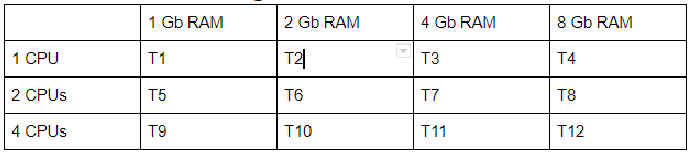
\includegraphics[scale=0.80]{images/tablesum.png}
    \captionof{figure}{\textbf{Figure \arabic{figure}:} Machine Configurations}
\end{center}

The result of the tests for Linux Servers, Linux Desktops, and Windows machiens are shown below, in Tables \ref{linserver}, \ref{lindesk}, and \ref{windows} respectively.

\begin{center}
    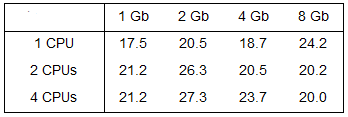
\includegraphics[scale=0.90]{DocumentationAndReports/Reports/images/linserver.png}
    \captionof{figure}{\textbf{Figure \arabic{figure}:} Linux Server Tests}
    \label{linserver}
\end{center}

\begin{center}
    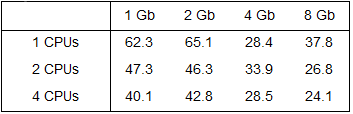
\includegraphics[scale=0.90]{DocumentationAndReports/Reports/images/lindesk.png}
    \captionof{figure}{\textbf{Figure \arabic{figure}:} Linux Desktop Tests}
    \label{lindesk}
\end{center}

\begin{center}
    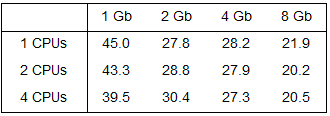
\includegraphics[scale=0.93]{DocumentationAndReports/Reports/images/windows.png}
    \captionof{figure}{\textbf{Figure \arabic{figure}:} Windows Tests}
    \label{windows}
\end{center}

\par From there, it was found through linear and quadratic fit tests that the time to build Linux Desktop and Windows machines were highly negatively correlated to the number of CPU cores. Those machines' times to build were also moderately negatively correlated to the amount of RAM available. In general, despite the higher correlation to CPU cores, those machines were much more effected by how much RAM was available. As can be seen in the above tables, machines with 8 GB or RAM could take half as long to build as machines with 1 GB of RAM, regardless of the number of CPU cores. Linux server machines were not well correlated with any of the variables tested. 

\par From there, six of the most popular Universities were surveyed to find their minimum computer specifications. We assume that many students follow those specifications and don't invest money in superior computers: in other words, an institutions minimum specifications are a good indicator of the hardware students are using. Looking at those Universities, we found that many students may use computers with only 4 GB of RAM and 2 cores in their CPU. Most students could dedicate 2 GB of RAM to a running virtual machine. Thus, Project BrightSun needs to work well under 2 GB of RAM and 2 CPU cores in order to meet Requirement 7.

\par As can be seen in Tables \ref{linserver}, \ref{lindesk}, and \ref{windows}, under those hardware specifications Linux servers take about 26 minutes to install, Linux Desktops take 46 minutes, and Windows Desktops take 29 minutes. These times are very inconvenient for users, and are a barrier to using our product. In order to make Project BrightSun easy to use and simple to set up (Requirement 2) we arbitrarily decided that all virtual machines should install in 30 minutes or less. Thus, Linux Desktop machines take much too long and Windows machines may take too long occasionally due to variance in build time. Therefore, we need to further investigate how to optimize the installation of virtual machines in order to meet product requirements. 

\par Furthermore, we have a benchmark for analyzing compliance with Requirement 7 in the future: if all virtual machines can build in under 30 minutes on 2 GB RAM and 2 CPU cores, we have met that product requirement. 

\par Our full analysis can be referenced for more details.

\section{Analysis of Project Need}

\par To ensure we were working towards the right goals with our project, we set out to determine the need for and theoretical efficacy of our tool as a solution to the problem initially identified.

\par To determine a need for our tool, we focused on the aspect of the established problem asserting that there is a shortage of well trained cybersecurity professionals in the workforce. To determine need, we analyzed findings from a Cisco cybersecurity report \cite{Cisco__annual_report} establishing that roughly 25 percent of surveyed cybersecurity professionals thought the number one problem in cybersecurity is a lack of trained personnel. With that statistic established, we examined the 2018 industry estimate of empty cybersecurity positions, 200,000 positions, compared to the projection for the next 4 years of up to 2.5 million empty positions. We determined that with the high percentage of professionals citing a lack of trained personnel to be the current biggest weakness in the industry, the massive projected growth of empty positions would greatly weaken the strength of the industry at large, justifying a need for an increase in the rate of new cybersecurity personnel entering the workforce.

\par Once need for an increase in cybersecurity personnel entering the workforce was established, we needed to perform an analysis to determine if our product would be effective at promoting an increased rate of entry through its use as an education device for young people interested in the field. To determine the affect of early involvement in cybersecurity on the education and career goals of those involved, we analyzed data from a US Air-force CyberPatriot program impact report \cite{cyberpatriot}, assuming that participation in the program was relatively representative of participation in easy-to-access cybersecurity learning and practice activities as a whole. The report provided statistics for CyberPatriot participants and alumni regarding their post-secondary-school education and careers, as well as the extent to which participation in CyberPatriot influenced their education and career goals. The data regarding the influence of the program was taken and aggregated into a scalar to represent an average impact of the program on a participant. The rest of the data in the report was processed via multiplication of the raw data by that impact scalar to create data which conservatively represented causality between participation in the program and career and education outcomes. Findings indicated a causal link between participation in the program and entry into a 4 year degree program for ~59.4 percent of respondents. Causality was also established for ~55 percent of respondents who went on to seek employment in computer science and cybersecurity, as well as for ~41 percent of respondents who chose a computer science or cybersecurity related major in college. From this analysis, we determined that there is a causal link between access to cybersecurity education and tools at a young age, thus justifying the educational goals of BrightSun in response to the problem addressed. 

\chapter{Iterative Approach}

\section{Usage of Scrum Project Management}

\par Delivering software with the correctly specified features, at the correct time, and at the planned cost is notoriously difficult. The example of the FBI’s Sentinel Project, a software case management system for the purpose of creating a digital management system for criminal cases, showcases this. Originally, the project was contracted out to Lockheed Martin as a several year endeavor costing hundreds of millions of dollars, with the traditional "waterfall" approach, where a centralized directive is given for the overall goal, and then Requirement Gathering, System design, Implementation, Testing, Deployment, and Maintenance, follow. Each step in the process is not started until the proceeding step is completed. This has the distinct disadvantages that once a mistake in a previous step is found, the work on later steps are likely worthless, and that by delaying testing of the interconnected system any interfacing errors are unlikely to be found until substantially work has been based on those earlier decisions{\cite{scrumFBI}}.  This is what happened with the Sentinel Project, where after reaching its due date, the new system failed to perform. The FBI then decided to drop Lockheed, in-source the development, and switch from Waterfall to Scrum project management. Then, in just 18 months after with less than one fifth of the original amount of developers, they rolled out the successful project. {\cite{scrumFBI}}. The reason for a successful project launch was a change from a Waterfall style to Scrum style approach to project management.

\par The Scrum system revolves around malleable project requirements that can be easily changed and acted upon based on customer input. Every week the development team plans out what they wish to accomplish that week, implement the deliverable, and evaluates the results with the customer for feedback. This is called a ‘Sprint’. Ideas are continuously developed through the project’s lifespan: the weekly planning meeting is a time where new ideas can be discussed among the group, and they can be pursued during the weekly sprint. Through this process, ideas not discovered during the pre-development brainstorming process can still be implemented into the project. For our project these weekly meetings were to gather our reactions to the week's work and ways to improve the process; then we were given opportunities to showcase progress made, and gauge the reaction of various individuals, from professionals, to professors, even the head of the UVA Cybersecurity team. We then held our second weekly meeting to address the concerns raised, or suggestions proffered, and decide on the path of development for the following week. This allowed us to change focus towards implementing a virtual box installer for enabling practice of novice users, and not towards establishing software which simulated system connectivity, based on the described difficulty. 




\subsection{Perspective: Beginning Scrum User}
\par As someone who had never used nor heard of Scrum before this project, I was intrigued by the fluidity of the project management style. From experience with prior projects, I was accustomed to planning things out from start to finish ahead of time, often having to set vague or unrealistic goals for the future due to a lack of initial information about the subject-matter and the difficulties to be faced. When faced with unexpected methods and directions to take such projects, it would be hard to adapt without discarding the entire initial planning scheme. These are the cases wherein traditional project management fails which were directly addressed by Scrum. 

\par Having gone into the project without prior experience in many of the technologies used, I was immediately struck by how productive and aimed we were able to operate within the first week-long sprint alone. Since there wasn't any need to create concrete long term plans and adhere to them, I didn't have to worry about trying to plan around concepts with which I was not yet familiar. Our development team met, laid out a set of tasks or "issues" to complete for the coming sprint, and were immediately able to start working. Any longer term ideas were put into a backlog to address when we were more suited to and we began instantly working on creating a deliverable product. This drastically different development approach kept me inherently more motivated and invested than traditional styles as I was always working on generating a product and everything I learned was instantly applicable to the build, providing frequent gratification through the tangible effects of my work. 

\par The use of Scrum allowed us fantastic flexibility throughout the project. Whereas new ideas and directions would be difficult to implement in traditional project management styles, we actively sought them out while using Scrum, which I believe to be one of the most integral elements to the success of our project. Meeting frequently with customers and amongst ourselves ensured that we were always on the same page and that we were always focusing our development on providing the greatest utility through our product to the people who would actually be using it. Unexpectedly to myself, that benefit of Scrum also played a large role in bolstering morale, as there was never a time when any of our work felt even slightly purposeless. 

\par As a first time Scrum user, I vastly enjoyed the opportunity to learn and use Scrum throughout this project. Scrum inherently fosters a sense of purpose, drive, and teamwork when properly implemented and I am eager to apply Scrum techniques in a multitude of projects going forward. 

\subsection{Perspective: Experienced Scrum User}

\par As someone who has actively used Scrum for several years and holds multiple project management certifications, I always enjoy having the opportunity to utilize Scrum on a project. With this project in particular, it was neat to see the team develop over the course of the semester through our Sprint Retrospectives. At the end of each sprint, in addition to analyzing our new product increment, we also evaluated our effectiveness as a team. Then, we would take a subset of those problems and build them into the following week's sprint as tasks in order to ensure we actually changed from our mistakes. 
\newline

``Lessons Learned that are never again looked at are not Lessons Learned. They are Lessons Documented.''
\\[5pt]
\rightline{{\rm --- Jake Smith}}\newline

\noindent More often than not in my previous Scrum teams, we have rarely implemented actionable changes from our retrospectives, so seeing our team self-critique and change throughout the semester has been a powerful experience. 

\par Additionally, another problem I have usually faced is with estimating the amount of work one can complete in any given week. In the past, estimates have been widely off-base, with our Scrum team consistently overestimating the amount of work we would be able to complete. Thus, for this project, we made conscious decisions about what we would actually be able to complete in the coming Sprint. These efforts enabled us to establish a continuous rhythm each week - momentum - independent of and taking into account our team members' other obligations. In the beginning we generally failed to do a good job of this, but in the mid to later sprints, we found our stride, regularly setting and hitting the specified goal for each sprint. In doing so, this project has been an excellent reinforcement of one of the core foundations of Scrum - shortening the feedback loop to maximize impact. Going forward, I will continue to look to apply both our successes and pain points on future Agile projects, both in school and in the workforce.

\subsection{GitHub Project Management}

\par Managing the project on GitHub was key to the success of Project BrightSun so far. The versatile tools GitHub makes available perfectly suited our Scrum approach and enabled us to work independently during times of high work load while keeping organized. These tools were new to most of the team members, but have all ready been incorporated into other projects.

\par One of the basic features of GitHub is the ability to list "issues". An issue is generally a task that needs doing, and includes metadata such as what the tasks involves, who the tasks is assigned to, and even commends and discussions regarding the issue. We used issues to list out goals for each Sprint, as well as to keep track of what features we want to implement in the future. Any bugs found have also been listed as issues so that we can either fix them in the future or help others mitigate their effects. 

\par Example issues from our project include "Functional Download Button", "Coordinate, early in the week, times to meet for cooperative work", and "Firewall breaks Packer". During the course of the project, 79 issues were closed and 29 are still open, including three feature backlogs. Below can be seen some of the current open issues. Note that the colored tags provide information on what the issue involves, and the small icons to the right show who has been assigned to the issue.

\begin{center}
    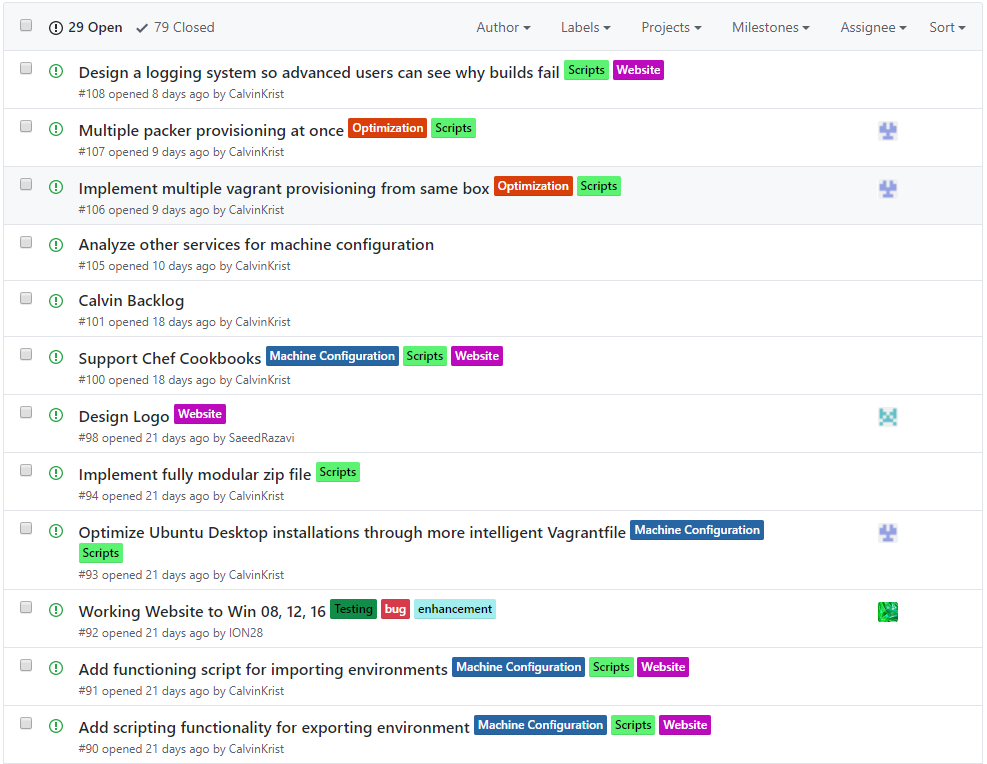
\includegraphics[scale=0.54]{images/issues.png}
    \captionof{figure}{\textbf{Figure \arabic{figure}:} GitHub Issues}
\end{center}

\par The ability to have discussions regarding an issue allowed us to work together on issues remotely. This was not of much value this semester, but over the summer could prove very valuable. It connects all discussion regarding an issue directly to that issue, which talking in a group chat does not do. Furthermore, it can allow people to post error logs or other key information that allows others to help de-bug. This may be a key element in the continuing project management of BrightSun.

\par Issues can also be assigned to "Projects" and "Milestones". These are how we organized our sprints for each week. An issue would be created and added to that weeks project and milestone. From there, any project member can see who is working on what issue, what the progress is, and what still needs to be completed for the week. As can be seen, all that is left for this sprint is for Saeed to finish designing a logo for Project BrightSun. 

\begin{center}
    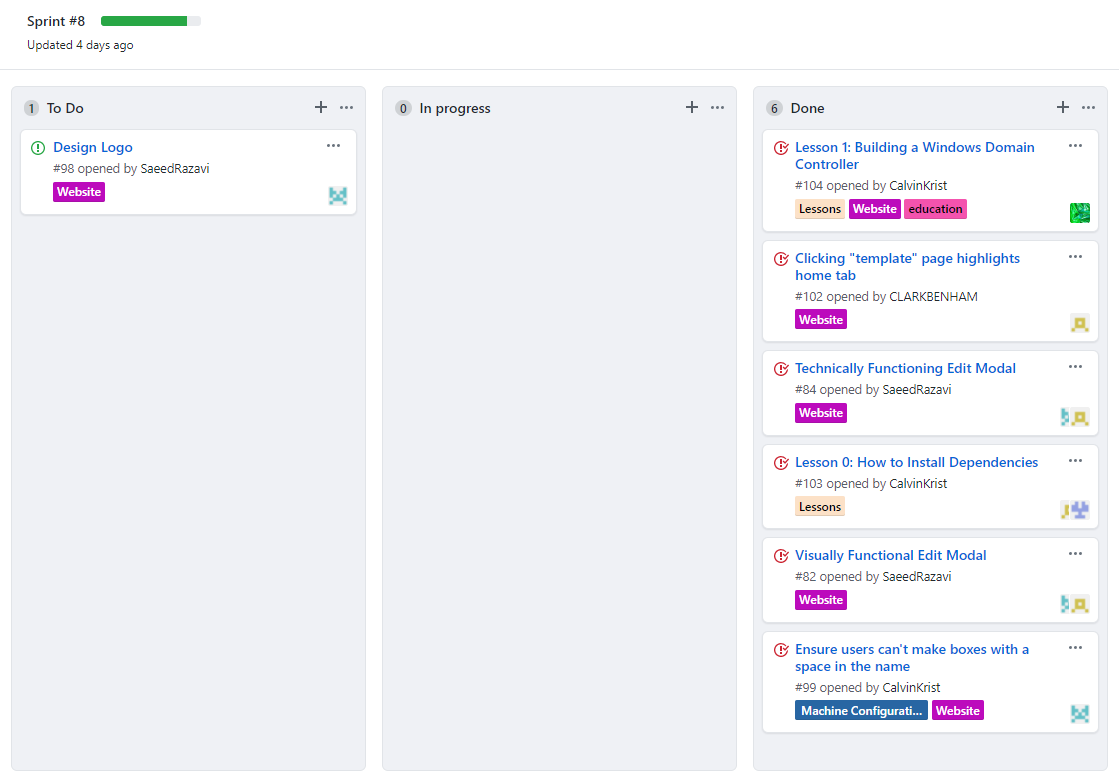
\includegraphics[scale=0.60]{images/project.png}
    \captionof{figure}{\textbf{Figure \arabic{figure}:} GitHub Project}
\end{center}

\par Throughout the course of this project, we found ourselves becoming much better at spacing out each sprint's work throughout the week. We also got better at judging how much work we could do and only assigning ourselves that much. These were both issues at the start of the semester, when the last couple of days before the end of a sprint were a much rush to finish everything. Our ability to pace our work can be seen in the below graph, which plots how many issues were left each day throughout a sprint. Our progress was very linear, which is exactly what we want.

\begin{center}
    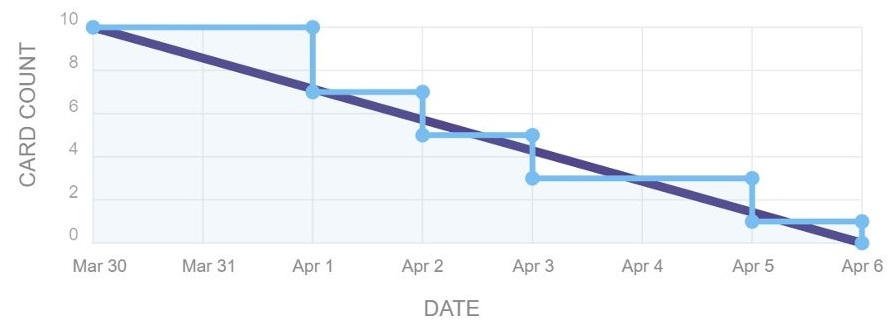
\includegraphics[scale=0.54]{images/throughput.jpg}
    \captionof{figure}{\textbf{Figure \arabic{figure}:} Sprint Progress vs Time}
\end{center}

\par Finally, projects can be released upon their creation. This has two main benefits: it allows for an easy overview of the time line of our project, and also preserves old versions of the project. That is very important because it allows us to revert to earlier versions of something breaks.

\section{Major Iteration 1: POC - Automated Virtualization}
\par There were two main goals Iteration 1: to test if it was possible to automate the building of virtualized operating systems, and to learn basic website design by making a demo local website. We needed to see if it was possible to automatically build virtual machines because that is the core product we are making. It is directly related to product Requirements 1 (machine apathetic), 2 (simple to set up), and 3 (models real world applications). If this was not possible with current technology, we would need to rethink our approach to the problem. In other words, Iteration 1 was about proving the feasibility of our project. We also prioritized learning and starting website development because those skills are what turn a series of files and scripts into an actual product that can be shown to customers, meeting product Requirement 2, simple to set up, and Requirement 4, teached cybersecurity effectively. It is the website, built on top of virtual machine automation technology, that could make Project BrightSun an easy to use learning tool. Otherwise, all we have made are a series of confusing and hard to use scripts. 
\par Iteration 1 was achieved in four weeks.

\par In order to see if automated virtual machine creation is possible, we drew upon Packer and Vagrant, two technologies discussed in our Phase I/II report. These technologies were chosen due to their ability to work on any operating system, which was a key product requirement, and their relative easy of use. Packer takes in a configuration file, specified in the command line, and can output a '\textit{.box}' file which represents a virtual machine. Vagrant can then take that '.box' file and mount it on VirtualBox, the application we use for interacting with virtual machines. This process can be seen in the figure below, where boxes represent files and arrows represent programs and processes.

\begin{center}
    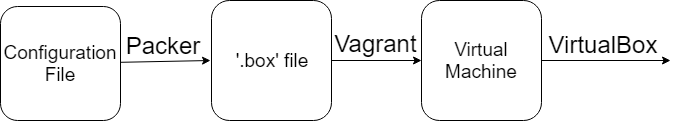
\includegraphics[scale=0.64]{images/Proto1.png}
    \captionof{figure}{\textbf{Figure \arabic{figure}:} Increment 1 Flow Chart}
\end{center}

\par At the end of this first increment, we saw that we could automatically build virtual machines. We also had semi-working configuration files for all of the major operating systems we chose to support (see Appendices: Operating Systems). However, we did not implement the full automation: we just knew it was possible. We still needed to manually specify for Packer in the command line which configuration file we wanted to use. Furthermore, the \textit{Vagrantfile}, a type of configuration file for Vagrant, still needed to be generated each time a virtual machine was created. But we knew that both of these tasks could be done by a simple script. Thus, what we had done at this point was implement the promise of Packer and Vagrant. It was time to start building on top of that.

\par Half of our group spent the first increment learning about website design and building a demo website. The website was meant to synthesize what the students had been learning while also giving a visual prototype for the '\textit{theme}' the website would have later. A website's theme is a set of visual features and layout choices that are independent of the actual website content. This may include a color scheme, where the navigation bar is located, how the website scales at different screen resolutions, or even if there's a drop shadow behind webpage elements. These two purposes can be well demonstrated in the figure below, showing the 'Home Page' of this demo website.

\begin{center}
    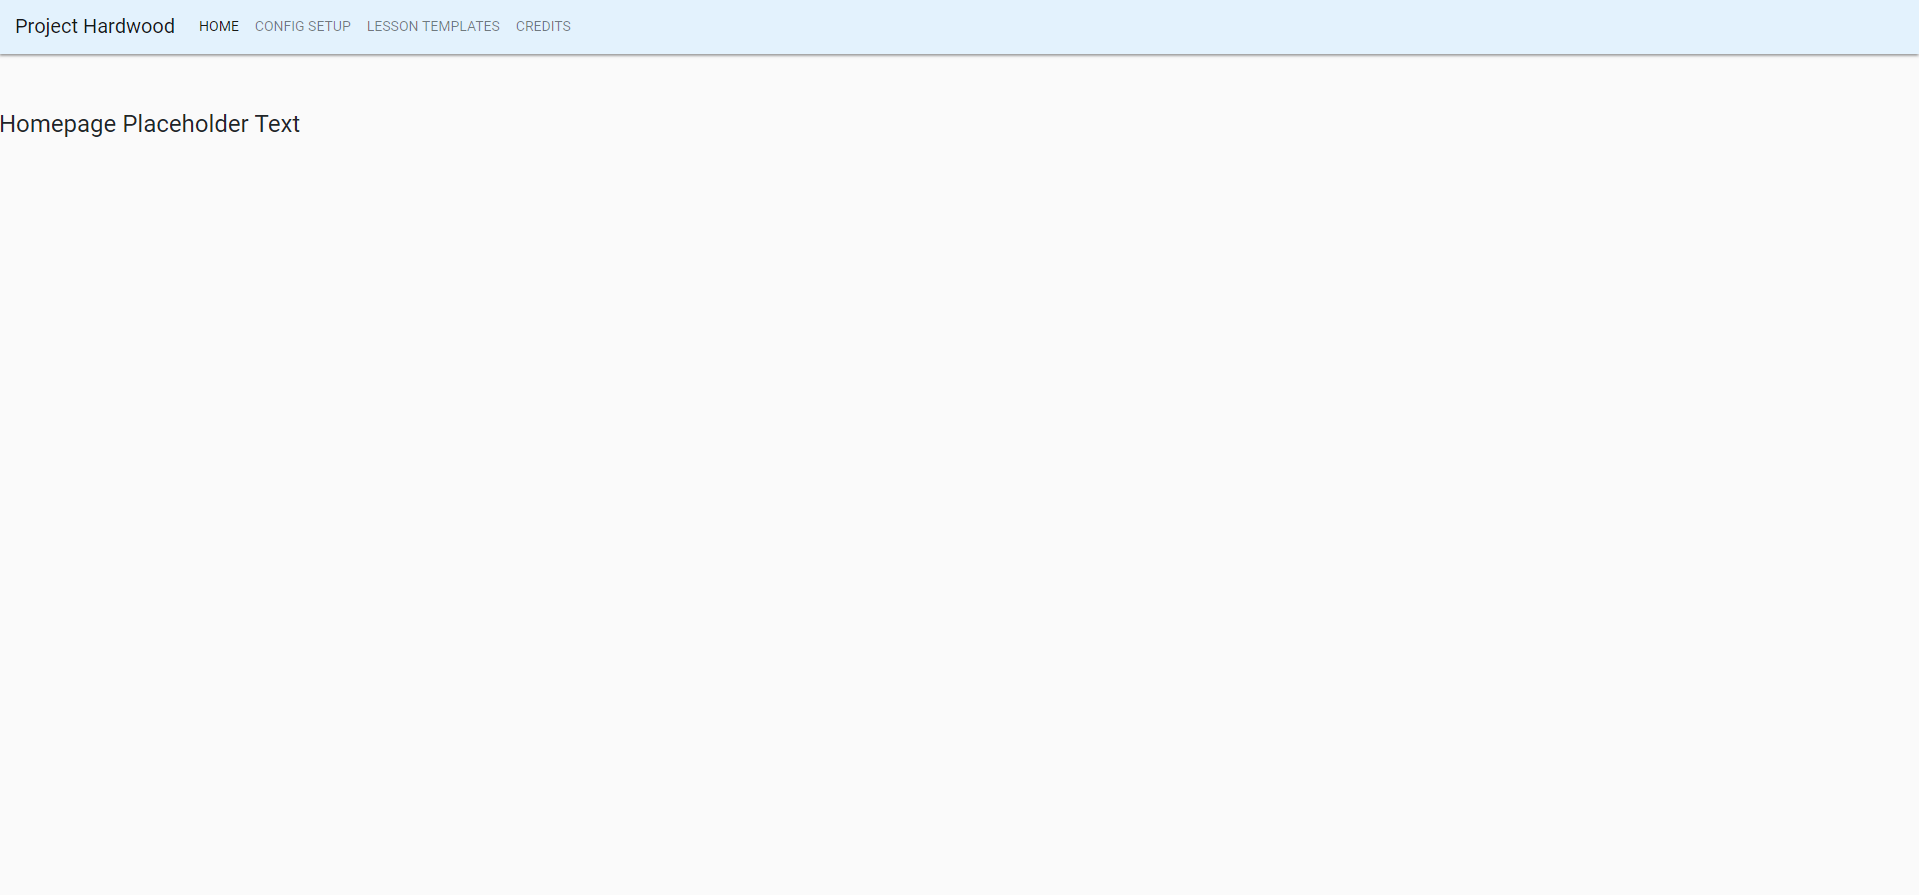
\includegraphics[scale=0.36]{images/homepage1.png}
    \captionof{figure}{\textbf{Figure \arabic{figure}:} Increment 1 Home Page}
\end{center}

\par The 'Home Page' was largely unappealing white space that served no functional purpose. However, it demonstrated that the students had learned how to make a web page. Furthermore, the navigation bar at the top visually shows a lot of the features of the website theme that have remained. The drop shadow below the navigation bar is still a noticeable design feature in our product. Furthermore, the general layout of the navigation bar has remained unchanged, with each of the website pages aligned linearly along the top. Thus, the website fulfilled both of its purposes by giving us a basic visual prototype and synthesizing the knowledge the students had developed during the first increment.

\section{Major Iteration 2: POC -  Website and Virtualization Integration}
\par The goals of Iteration 2 were to create more versatile virtual machine provisioning, find the easiest way for users to create a virtual machine on the website, and link the website to the Packer scripts developed earlier in an automated manner. In other words, by the end of the second iteration we wanted a website that could be used for automatic virtual machine creation. These goals were completed in three weeks.
% Why did we have these goals?
% >Find the easiest way for users to create a virtual machine on the website:
%   >>Machine cards on left, new machine box on right with checkable options
%       >>>Unintuitive - very much a first pass design with good bones
%   >>Machine cards in main space, add new and download buttons in top corner with pop-up options modal (utilizes dropdowns)
%       >>>Easy to see what machines you have
%       >>>Fairly intuitive generation
%   >>Drag and drop prepared machines with naming options
%       >>>Very easy and intuitive
%       >>>Limiting in possibilities
%   >>Conclusion of which to use as a basis
%       >>>Already stated in report. Maybe just flesh out with the fleshing out of above ideas
% >Link the website to the Packer scripts developed earlier in an automated manner
%   >>This section is pretty well explained and I don't really think it needs much more. Perhaps discuss what led to the decision that this work around was the best (although we clearly just went with it because it made sense - get more team input here)
% >Broadly:
%   >>We would create a product resembling the shell of the minimum viable product to be fleshed out and given function in future development
\par First, we made the virtual machine provisioning more versatile. At the end of Iteration One, virtual machines could be made using Packer and Vagrant, but an Ubuntu 16.04 machine was always the same machine. In other words, users couldn't install custom software, or configure the machine to suit their needs. Thus, it had very little use as either a professional or a learning tool, failing both Requirement 3 (models real world applications) and Requirement 4 (teaches cybersecurity effectively). One of the main strengths of where we see our product going is that a wide variety of users can adapt it to suit their needs. In many ways, that is \textit{all} we are trying to accomplish: making a versatile method of automatically generating virtual environments. Thus, having the ability to customize the virtual environments is absolutely necessary, and this comes by supporting custom provisioning at both the Packer and Vagrant level. During Iteration 2, we were able to implement custom provisioning at the Packer level, meaning that users can create any number of virtual machines with custom scripts run. When Packer is used to generate `.box' files, additional custom provisioner scripts are executed. Users could modify these scripts to suit their own needs and, in the future, the scripts will be modifiable using the website. The figure below shows the new process for creating virtual machines.

\begin{center}
    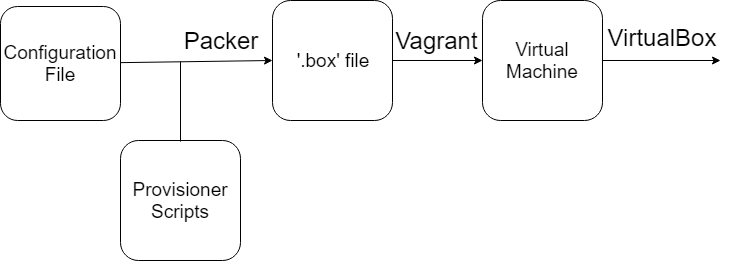
\includegraphics[scale=0.64]{images/Proto2.png}
    \captionof{figure}{\textbf{Figure \arabic{figure}:} Increment 2 VM Flow Chart}
    \label{scriptFlow}
\end{center}

\par The next step was to determine how users would create virtual machines using our website. In order to help answer this question, we drew three different design ideas for what a "virtual machine creation" page might look like. The first design is shown below.

\begin{center}
    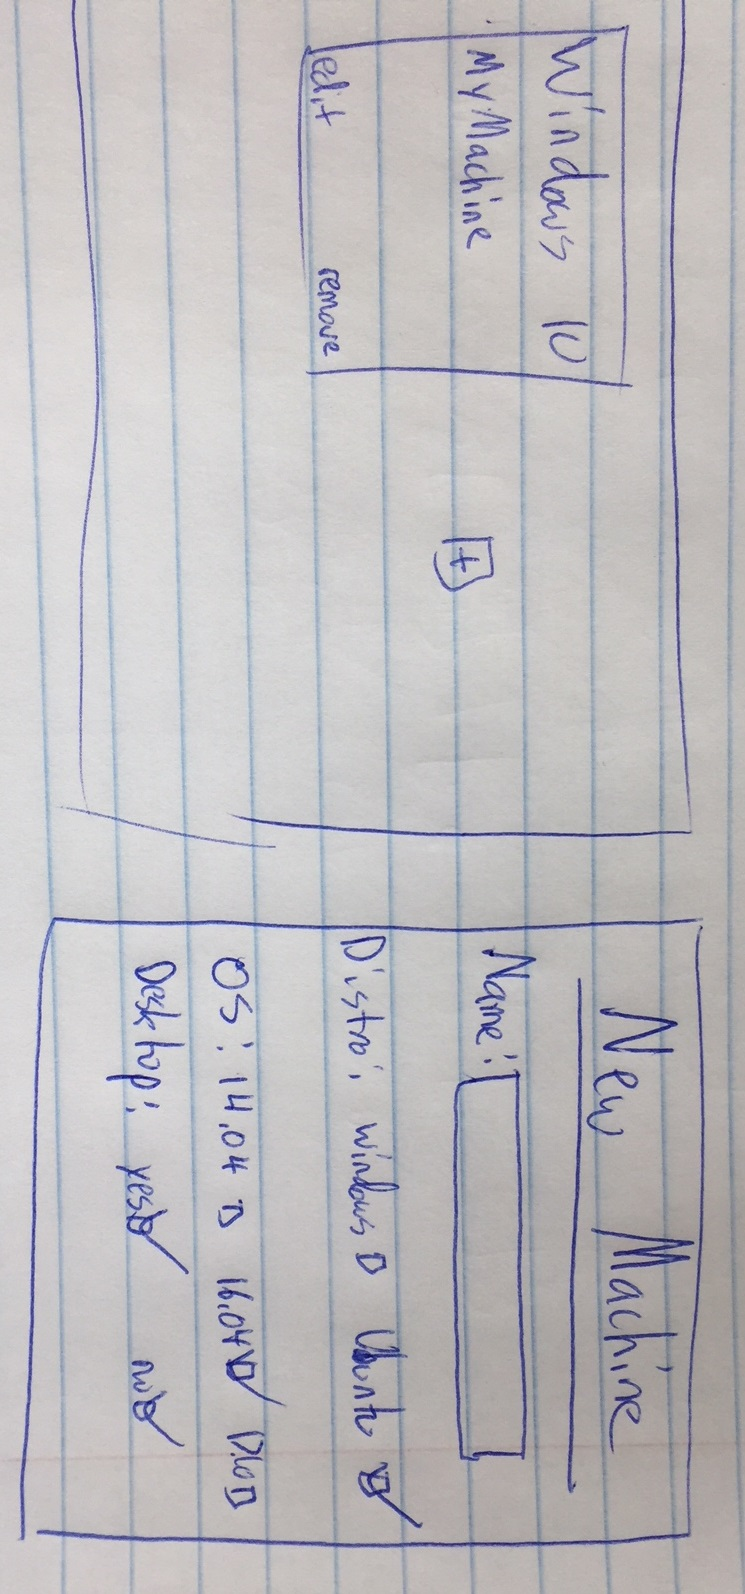
\includegraphics[scale=0.27, angle=90]{images/design2.JPG}
    \captionof{figure}{\textbf{Figure \arabic{figure}:} VM Creation Page Design 1}
    \label{design1}
\end{center}

\par The design centers around a window displaying the machines the user wants to create, seen in the left of the figure. Basic information is given about the machine for the user to see, including which operating system it is and what the user named it. More information such as the RAM dedicated to the machine would clutter the GUI. The user has the options to edit or delete the machine. There is also a box with a `+' in it where the user can add another machine. The box to the right of the figure is what the user might see when adding a new machine. A series of simple check boxes allows the user to select what machine they want to create.

\par Our second design is a slight variation on the first. We kept the window displaying the created machines, but removed the '+' for adding new machines and created a button at the top right label "Add New" as well as a download button. This design can be seen below.

\begin{center}
    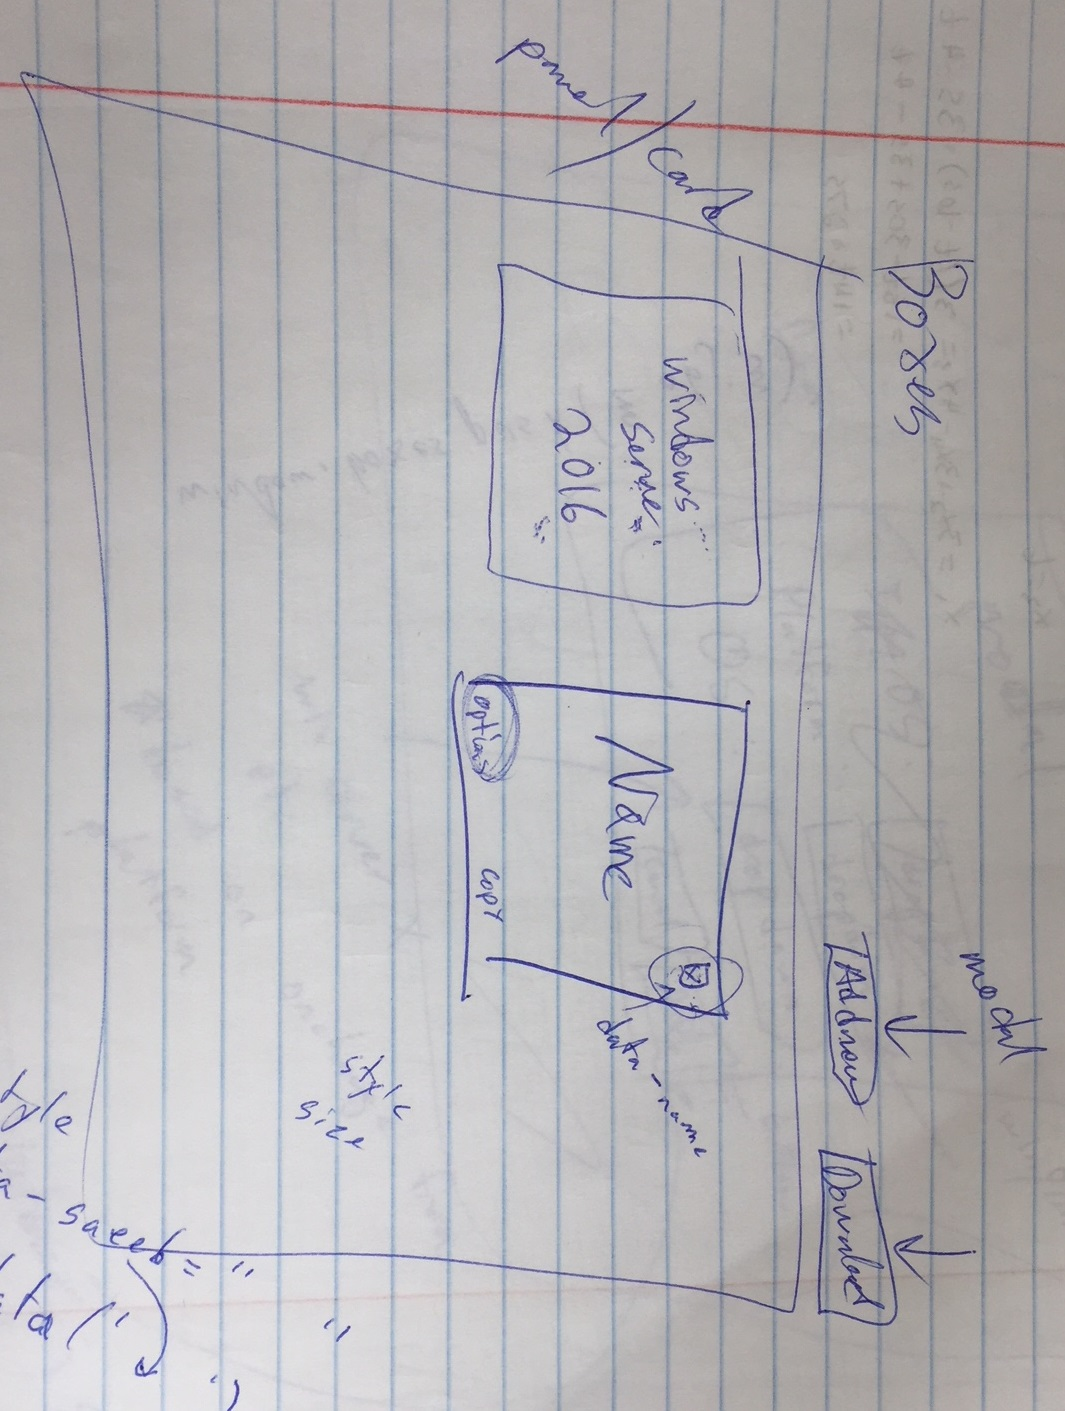
\includegraphics[scale=0.25, angle=90]{images/mainDesign.JPG}
    \captionof{figure}{\textbf{Figure \arabic{figure}:} VM Creation Page Design 2}
    \label{design2}
\end{center}

\par We also re-designed the window for creating new machines, seen below. The new design uses drop down menus instead of check boxes in order to reduce clutter.

\begin{center}
    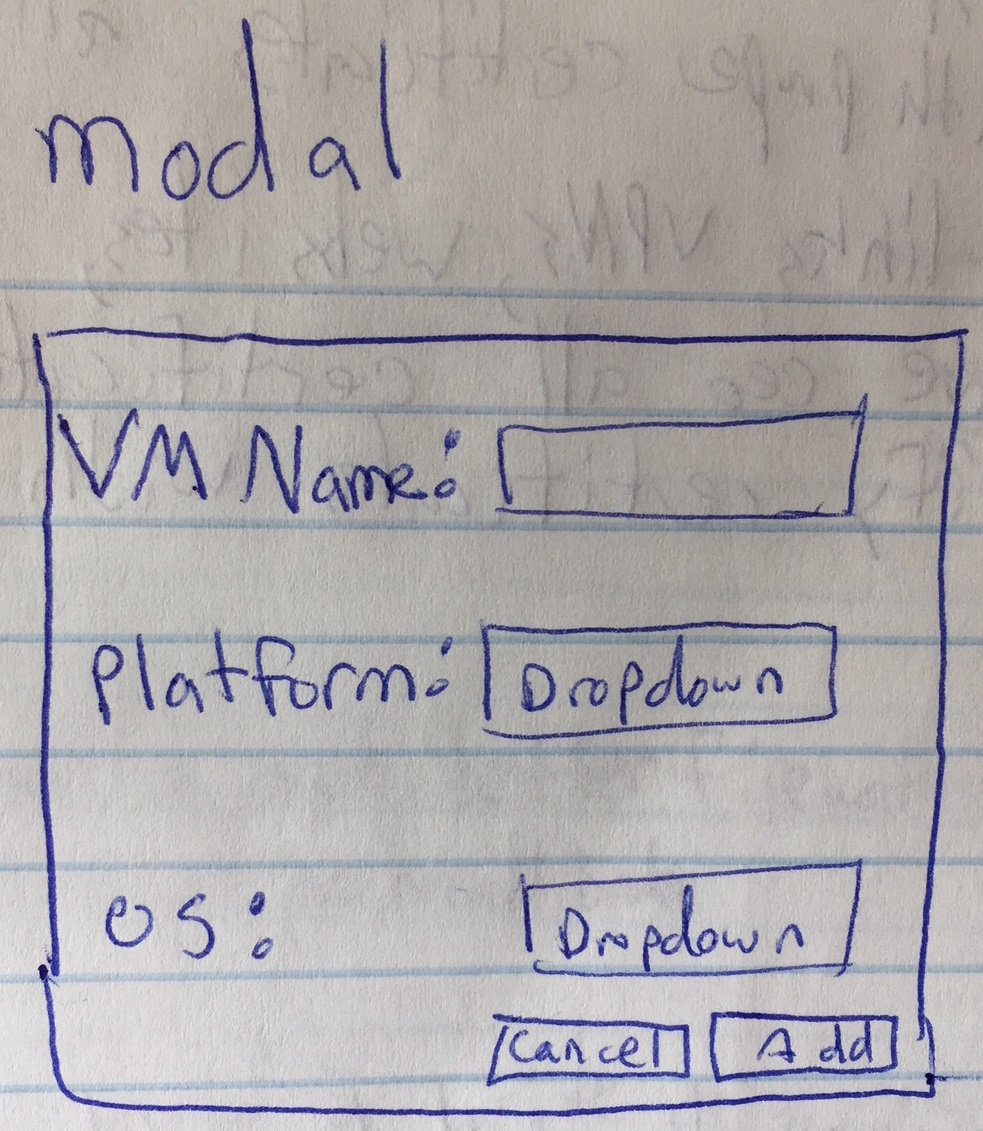
\includegraphics[scale=0.22]{images/modalDesign.JPG}
    \captionof{figure}{\textbf{Figure \arabic{figure}:} VM Creation Window Re-design}
    \label{newModal}
\end{center}

\par Our final design used a more drag-and-drop approach, where users could see the possible virtual machines on the right and drag them to a shopping-cart type setup on the left. This design completely avoids the separate window for creating a virtual machine, making is a little more intuitive to use.

\begin{center}
    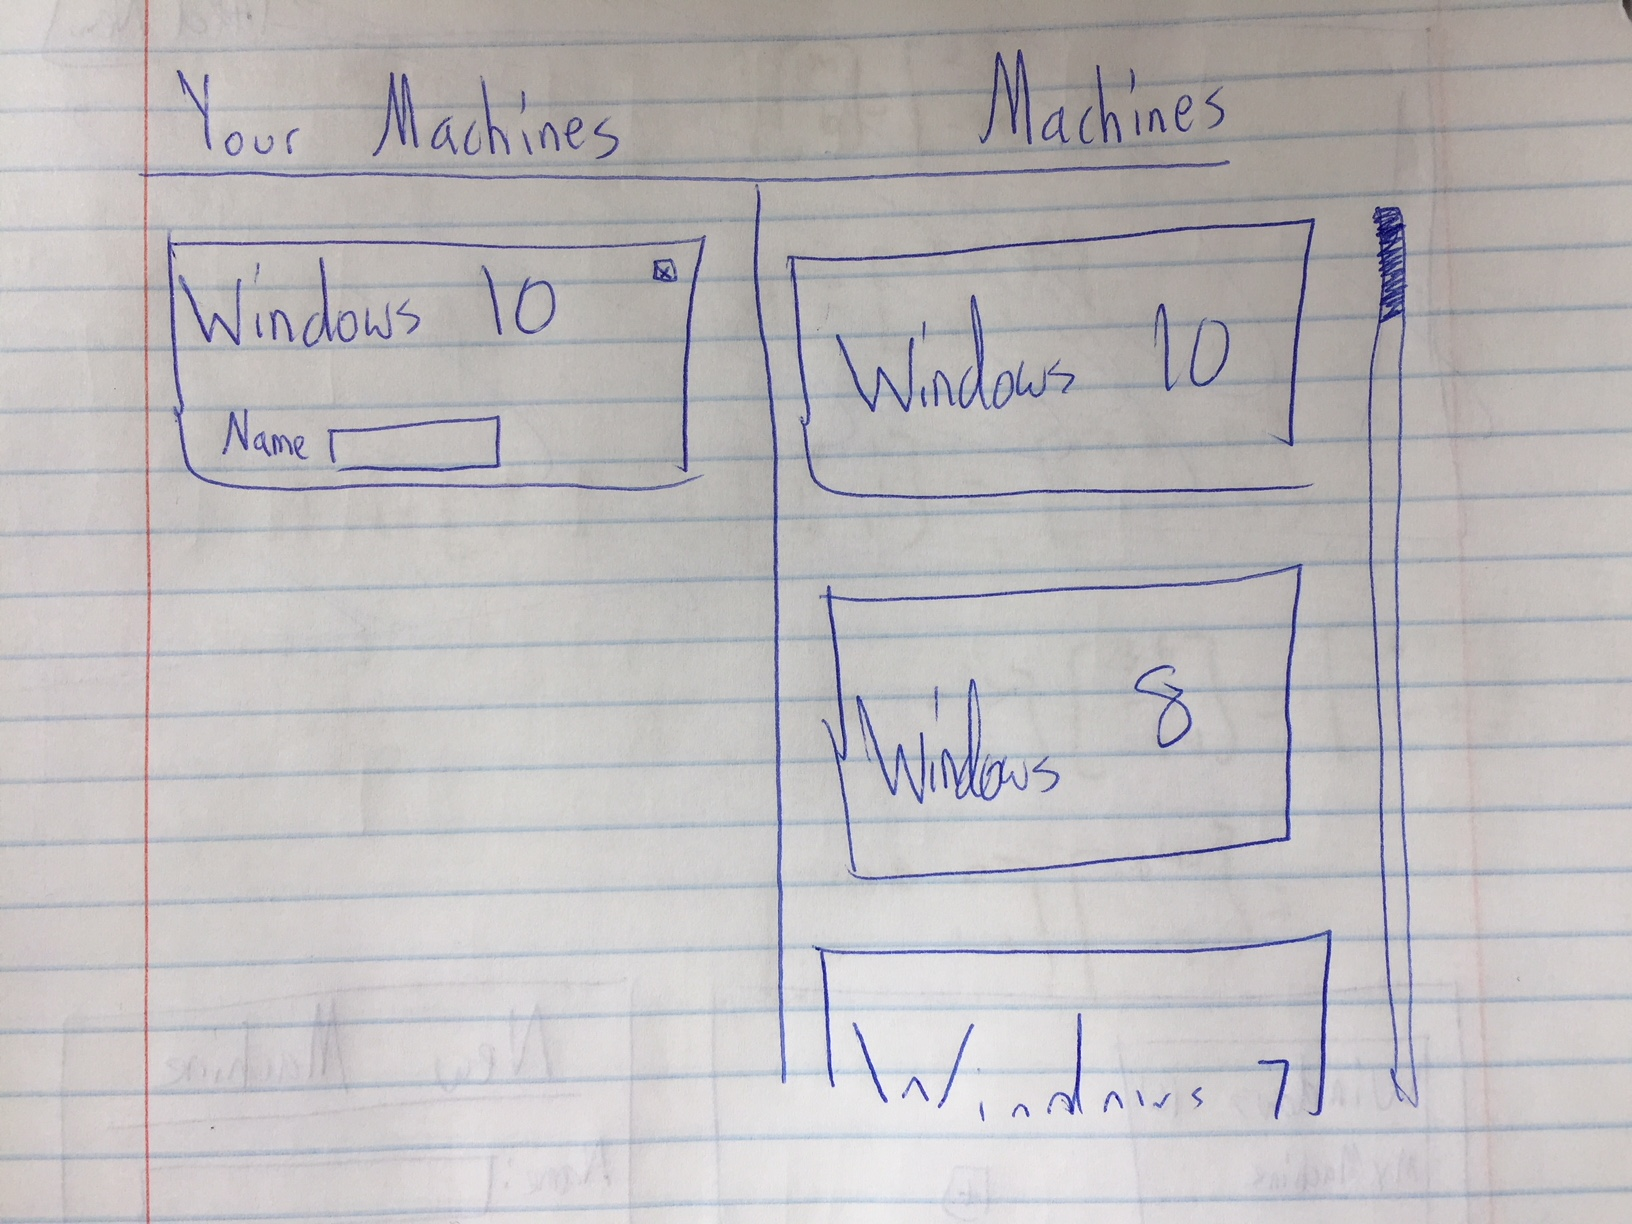
\includegraphics[scale=0.24]{images/design3.JPG}
    \captionof{figure}{\textbf{Figure \arabic{figure}:} VM Creation Page Design 3}
\end{center}

\par The pros and cons of each design were discussed among our group. It was quickly decided that the second design of a VM Creation Window, seen in Figure \ref{newModal}: VM Creation Window Re-design was superior to the first. The drop down boxes were far less cluttered than the check boxes, making the design more visually appealing, and when we add support for more virtual machines in the future it will be easier to expand the design.

\par Between Designs 1 and 2, seen in Figures \ref{design1} and \ref{design2} respectively, the second was superior. The Design 1 used a `+' sign as an "Add New" button, which could be confusing to some users. Furthermore, it didn't have a "Download" button which was a glaring flaw -- without the ability to download virtual machines, the website is useless. One could have easily been added in the top right corner such as in Design 2, but at that point it would look best to add the "Add New" button next to the "Download" button and you now have Design 2.

\par Thus, it came down to a debate between Design 2 and Design 3. They were radically different designs that each had their own merits. Design 2 allowed the user to easily see which virtual machines they were going to download, and lent itself to users downloading multiple machines due to the large amount of space. Design 3 could only show three or four machines at a time, however. On the other hand, Design 3 was probably more intuitive to use due to its drag-and-drop nature, while Design 2 required users to navigate a separate menu in order to add a machine.

\begin{center}
    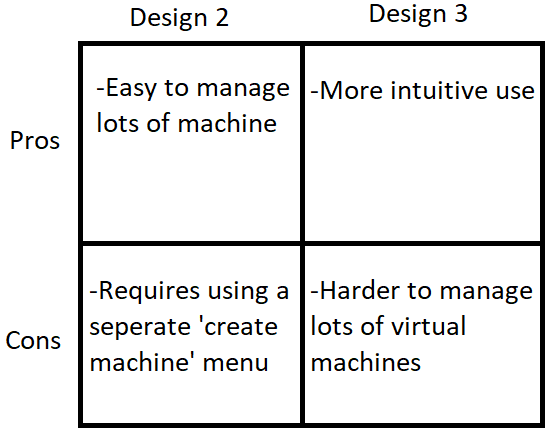
\includegraphics[scale=0.64]{images/proscons.png}
    \captionof{figure}{\textbf{Figure \arabic{figure}:} VM Creation Design 2 vs 3}
\end{center}

\par The decision was based on how we see our product being used. Most likely, Project BrightSun is best suited to situations where either complicated virtual machines need to be made or multi-machine, complicated virtual environments need to be created. In the second use case, Design 2 is easier to use than Design 3 due to its ability to allow users to see all of their machines at once. While we do hope many students will use our product, we don't expect the burden of navigating a separate menu for creating a virtual machine to be prohibitive.

\par Thus, we decided to implement Design 2. We did not implement multiple designs and give them to our customers to test due to how time prohibitive this would be. Each design would likely take two or three weeks to implement, and we decided the higher priority was getting a usable prototype to customers in order to get feedback. If the feedback had included difficulty navigating the virtual machine creation process, we would have re-designed the page.

\par The next step was to implement the virtual machine creation page and link it to our scripts. This happened simultaneously, where half of our group made the webpage and the other half worked on the back-end that connected the website to our scripts. Ideally, the user would set up their machines in the webpage, click a button that said "Build", and then wait half an hour while it built and provisioned the virtual machines. However, that was not easily possible.

\par Product Requirement 6 is to limit the number of applications the user must install to use Project BrightSun. As such, we could only use JavaScript to link the webpage to the scripts. Browsers limit what JavaScript can do for security purposes, meaning that even though it's a local website (not hosted on an external server) we are unable to run scripts directly from the website or to even read files from the computer. These are both large issues: the inability to run scripts from the website means user interaction is necessary and full automation from the website is impossible. The inability to read files from the computer means that we can't easily create a fully modular download that can be sent anywhere.

\par We did not spend much time trying to overcome this problem, because it can be easily fixed later and we wanted to get a minimum viable product completed before the project deadline. Potential solutions we came up with included converting all the dependant files to JavaScript so they could be directly downloaded or moving the local website to a server we host. Both of these were rejected due to feasibility concerns. We chose not to convert the dependant files to JavaScript because there are hundreds of files and it would take too long to convert them. Furthermore, if the files needed to be changed or updated it would be much more difficult. We never considered the idea of moving to a hosted website for long because one of the main project requirements is that there be no associated costs for any party involved, including us. Hosting a website would cost money that would either require placing ads to pay for that or charging customers. Neither option was acceptable.

\par Instead, the JavaScript back-end receives the machines the user wants from the website and generates most files the user needs, including some script files. The full process can be seen below in Figure \ref{fullBuild}.

\begin{center}
    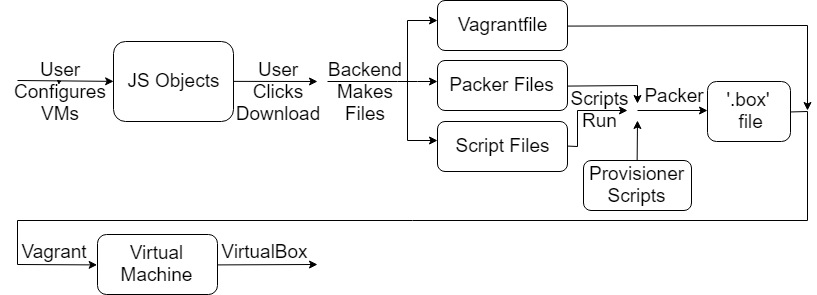
\includegraphics[scale=0.58]{images/fullDiagram.png}
    \captionof{figure}{\textbf{Figure \arabic{figure}:} Full Build Flow Chart}
    \label{fullBuild}
\end{center}

\par The back-end generates three main files: Packer files, which are used to configure the machine, a Vagrantfile, which is used to help Vagrant provision the machine and mount it in VirtualBox, and script files, which are used to automatically carry out all the steps described in Iteration 1 (such as running Packer through the command line). The files are then placed into the same directory as the dependencies, a step not shown in the figure, and the script is run. From here, everything happens in an automated fashion without user intervention. Packer uses the Packer files to know what machine to build as well as the provisioner scripts discussed earlier in Iteration 2 that allow for customized provisioning of the machine. Packer then outputs a `.box' file which is passed to Vagrant, which turns the `.box' and the Vagrantfile into a usable machine mounted in VirtualBox.

\par The configuration page for the website was created successfully and linked to the JavaScript back-end. Figure \ref{config} shows the configuration page with a couple of virtual machines added, while Figure \ref{modal} shows the menu for adding a new machine.

\begin{center}
    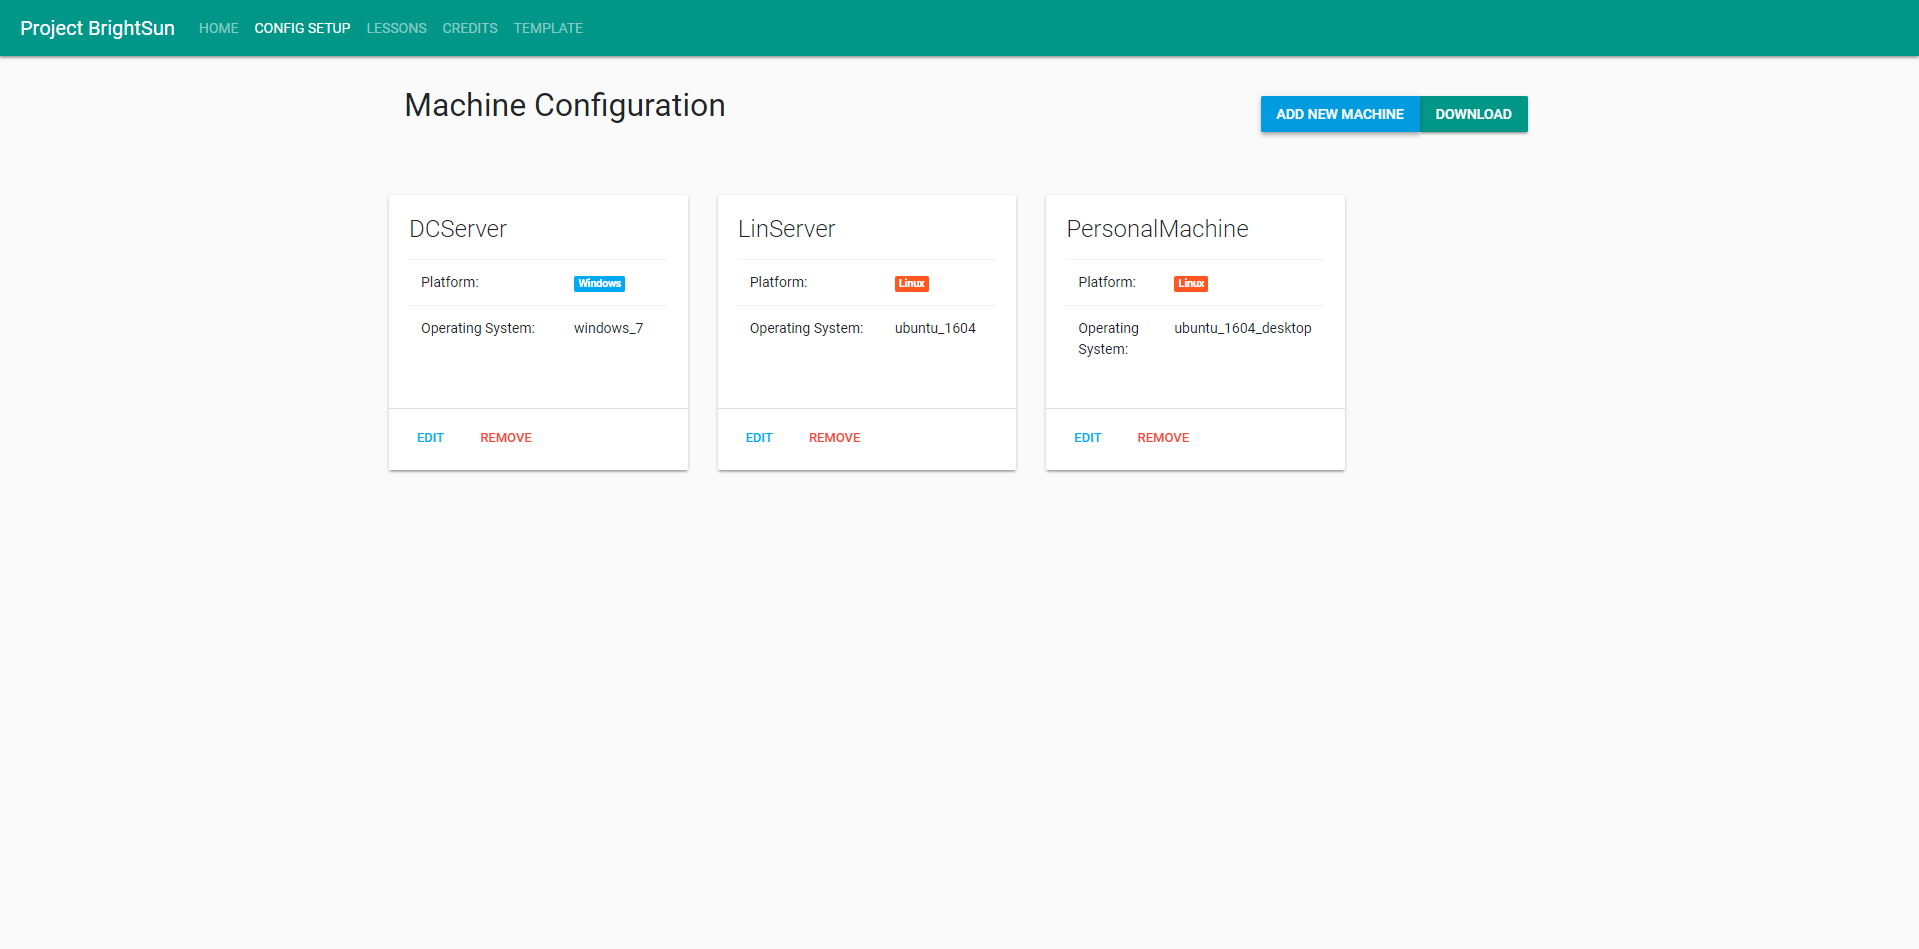
\includegraphics[scale=0.33]{images/machines.png}
    \captionof{figure}{\textbf{Figure \arabic{figure}:} Configuration Page}
    \label{config}
\end{center}

\begin{center}
    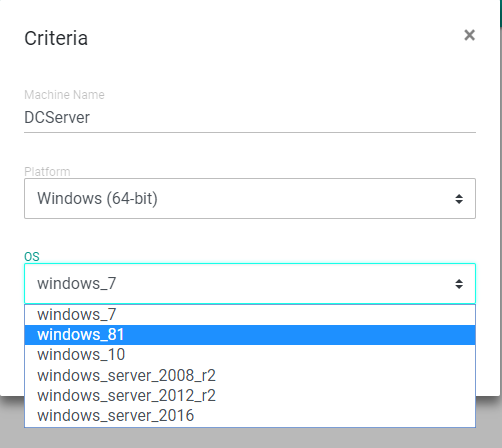
\includegraphics[scale=0.64]{images/modal.png}
    \captionof{figure}{\textbf{Figure \arabic{figure}:} Machine Creation Page}
    \label{modal}
\end{center}

\par The `edit' and `remove' buttons did not work, but users were able to add machines, download the necessary files, and then automatically install the machines. Our goals for Iteration 2 were achieved: we had support for versatile machine configuration, a configuration page was designed and implemented, and a back-end was created that more or less connected the script files made in Iteration 1 to the website; however, our web platform lacked support for lots of customizations and did not have a set of lessons for learning about cybersecurity like we initially envisioned.

\chapter{Current State: A Minimum Viable Product (MVP)}

\section{Overview}
After finishing Major Iteration 2, we had about 2 sprints remaining in the project. By this point, we had validation on both of the major components required for a final product: demand (we have identified problem, customers, and requirements) and technical feasibility (automating installation of virtual machines and downloading configurations through a website). In essence, we have reached what we consider to be a solid Minimum Viable Product (MVP) with our current state. Going forward from this point, we spent the final weeks of our project adding small features, enhancing the user experience, and building out the basis for our Lessons section.

\subsection{Linux Virtualization}

\subsubsection{Current Progress}

\par When we set out to do this project, we intended to offer support for the major Ubuntu distributions that are used. This includes Ubuntu 14.04, 16.04, 17.10, the dekstop versions of all of those, and the x32 bit versions of all of those. Successful automated installation was created for all except the 17.10 desktop. The virtual machines are created in about 20 minutes if they are a server and 20-60 minutes if a desktop, depending on the available hardware. Furthermore, there is support for customized provisioning user Packer, which will allow for customized installation and setup of any Linux machine. After they have been installed the first time, users can re-install the machines if they break in just a minute, making this already a valuable tool for week long labs in school.

\subsubsection{Future Work}

\par At its current state, there is a solid foundation to move forward with Linux machines. However, there are important features that we know users want that are missing:

\begin{itemize}
    \item While there is support for Packer custom provisioning, a library of pre-made scripts should be created or compiled to do many of the common tasks. This needs to include basic network tools and software packages.
    \item Installation times of Linux Desktop machines needs to be brought down to under 30 minutes on machines with 2 GB of RAM and 2 CPU cores in order to meet Requirement 7, low machine specifications
    \item The Linux machines supported should be abstracted in some manner to allow professionals to easily use Project BrightSun with Linux versions we don't currently support. This would work towards Requirement 1, machine apathy
\end{itemize}

\subsection{Windows Virtualization}

\subsubsection{Current Progress}
At our current state, we have support for the Windows versions listed in Appendix \ref{appendix:os}: Operating Systems. These are the 3 most recent versions of both regular Windows and Windows Server spanning the last 9 years. With each of these OSs, we have fully automated their install, enabling them to be automatically provisioned based on which version the user selects on the web interface. Within each install, we have abstracted most of the settings/features to easily configure them which allow further customization than just a base install. In addition, we have support for adding a custom list of user accounts to the machine as well as enabling any specific Windows Feature/Component. These steps represent the beginning framework in equipping the user with the ability to full customize any part of the install themselves.

\subsubsection{Future Work}
At its current state, we have a solid framework for Windows builds upon which we can continue to build. In the coming months, we will begin adding the items below which will enable further customization and more advanced environments to be created, all in an automated fashion through our platform.
\begin{itemize}
    \item Installation of specific software packages, ie hMailAdministrator, XAMPP, Cygwin, etc, in order to meet product Requirement 3, models real world applications.
    \item Windows Active Directory Domain Services, which is crucial for setting up business-like environments (Requirement 3).
    \item Ability to run custom scripts Powershell scripts on machine creation, enabling users to tweak additional settings on their own, in order to meet Requirement 1, machine apathy.
\end{itemize}

\subsection{Website Presentation}

\subsubsection{Current Progress}
At its current state, the Web Platform proves and validates our idea that a user should be able to fully customize and download a set of virtual machines that will be automatically provisioned. Right now, we have created each of the major pages of the site and at a minimum, a solid structure for those pages going forward. The core of the website lies in the configuration page which enables users to create a set of custom virtual machines. Users have the ability to select a name for the machine, platform (Linux or Windows), and finally, choose a specific operating system version. This process can be repeated as many times as necessary to download an entire cluster of machines. In addition, once the user is done creating machines, the build scripts can be downloaded and executed to automatically provision the machines based on the user's configuration.

\subsubsection{Future Work}
Right now, as similar to Windows, the current status of the web platform proves everything is possible, yet it lacks the ability to do complex machine and network configurations that would enable it to be truly useful in a classroom setting. Below are some of the features we plan to add next in order to fill in these gaps before getting it in the hands of students in a classroom setting (excluding for testing purposes):

\begin{itemize}
    \item Virtual machine settings, ie RAM, HDD size, VirtualBox Networking info, etc
    \item Integration of aforementioned Linux customization options
    \item Integration of aforementioned Windows customization options
    \item Support for importing and exporting virtual machine configurations. This is a feature we heard requested from lots of customers and works towards Requirement 2, simple to set up.
    \item Basic network control through a GUI. This is key to make networks easier for new students, meeting Requirements 2 (easy to set up) and 4 (good teaching tool). It also makes it easier to set up virtual environments, making Project BrightSun helpful to intermediate and advanced users due to modeling real world environments, Requirement 3.
\end{itemize}

\noindent Although these may seem small, we anticipate these items taking a considerable amount of effort in order to properly integrate and test all of these new features.

\subsection{Lesson Templates}

\subsubsection{Current Progress}
Since the beginning of the project, our goal has been to find new ways to enhance cybersecurity education. In following with this mission, we quickly realized that it would not be enough to simply provide a tool to automate installation of complex environments, but we should have some documentation and example lessons alongside it. These lessons would enable students to have some guided direction when starting out before tackling more complex subjects and conducting research on their own. Right now, we only have a few lessons put together, one for getting started with our platform, and another on how to set up your own Windows Domain Controller.

\begin{center}
    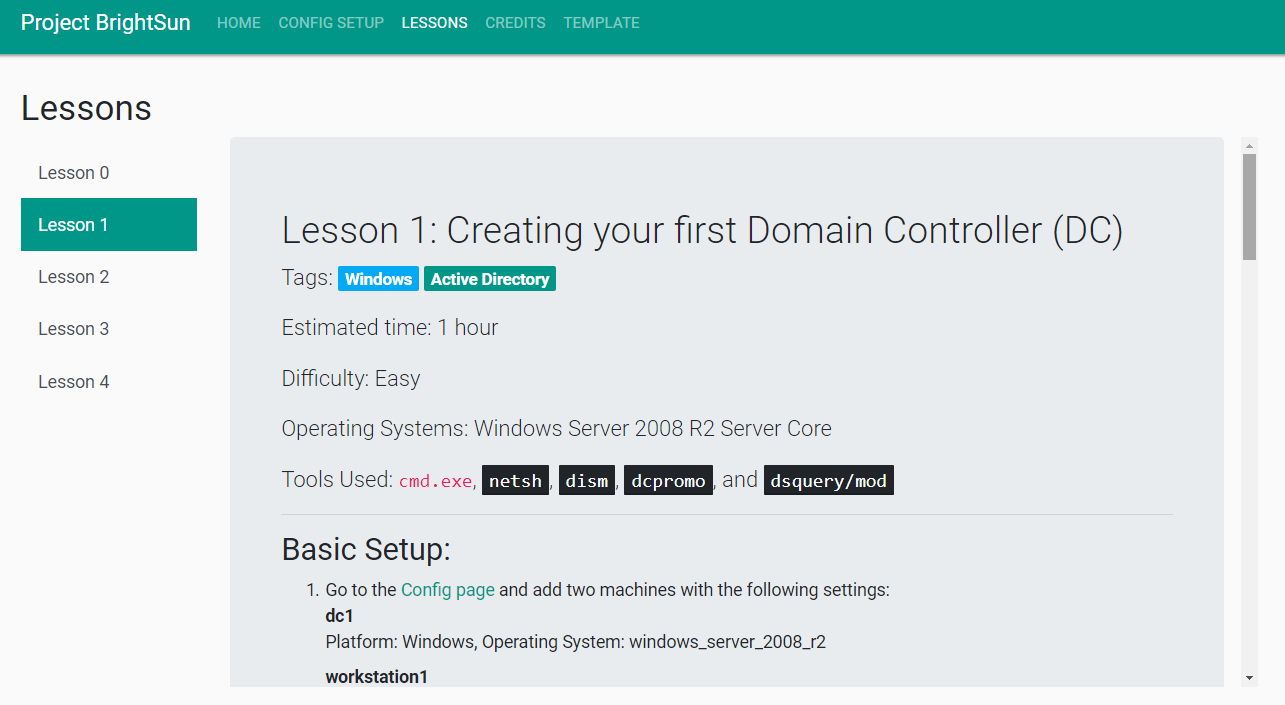
\includegraphics[scale=0.50]{images/lesson.png}
    \captionof{figure}{\textbf{Figure \arabic{figure}:} Lesson Page}
    \label{config}
\end{center}

\subsubsection{Future Work}
As we continue adding in more advanced customization options as described above, we plan to add more lessons that really highlight what our tool is capable of and focus on providing more introductory lessons/labs for key cybersecurity topics. For our student and teacher stakeholders, these lessons will both act as good starting points for lessons they can use in class / on their own as well as provide illustrate the benefits of our tool. Some future lessons we envision include:

\begin{itemize}
    \item Performing Golden and Silver Ticket attacks against Windows Active Directory Environments
    \item Lateral Movement across a Windows Network
    \item Managing and Securing Linux Users
    \item Attacking a Business Network (similar to the setups found in the Collegiate Cyber Defense Competition (CCDC)) 
\end{itemize}

Key to making these lessons effective is offering pre-built virtual environment configurations that can be imported into Project BrightSun. This would allow students to learn in environments that we provisioned specifically for a lesson.

\section{Future Plans}

Above we have mentioned all of the future work we have planned for the project from a technical perspective, but not if and how we will ever accomplish those goals. Although this paper acts as a close to the official end of our project from a purely academic project for Engineering 1420, we plan to continue working on this project through the summer and beyond in our spare time. In particular, we have already quantified how this project may help us prepare for next year's CCDC competition and teach workshops at the Computer and Network Security Club next semester. Beyond that, we envision one day where our tool is actually used in a classroom environment to help students learn cybersecurity. Although we won't have as strict a schedule moving forward, we are all really looking forward to continuing with the project.

\chapter{Risk Assessment}

\section{Design for Environmental Sustainability}

\par The main way our product could effect the environment is by changing how computers are used and how much they're used. For example, if our product results in more secure computers, people may trust computers more and hence use them more. 

\par Project BrightSun would only have an effect if it makes traction in the security community. There is no other likely route for environmental impact. While it is stored on GitHub servers, requiring silicon, electricity, and cooling, it is a very small project consuming few resources. It will hopefully encourage more people to pursue a cybersecurity career, but those people were likely interested in computer science already, so that occurrence would not result in a significant increased use of computers. If our product makes no traction in the security or educational communities, it will likely make none in the criminal community either. Thus, even if Project BrightSun doesn't make IoT devices safer it won't make them \textit{less} safe. We are left with our product effecting the environment only by changing how computers are used.

\par There are four main categories of computers in the present day: personal computers, servers, smartphones, and embedded devices / IoT computers. Personal computers are desktops and laptops, the types of computers the general public uses for work and personal purposes. Servers are used to host large databases and other services. This is often colloquially referred to as "the Cloud", and includes things such as Google Drive, Twitter, and really most of the Internet. Smart phones are phones, generally pocket sized, that operate on top of a computer and allow the user to use the device through a GUI. Embedded devices / IoT are the computers in cars, in smart coffee machines, in security cameras: these are the small, cheap computers that control many every day devices. There are currently about 25 \textit{billion} embedded / IoT devices, and this number is projected to continue growing at an exponential rate \cite{iot_numbers}. 

\par How could our product change computing behaviours in any of those categories? Servers use lots of electricity, and the high quality hardware they run on requires lots of silicon \cite{datacenter_energy}. Both of those resources are damaging for the environment. However, our product would not change the usage of either of those resources. Servers are necessary for businesses, and as such security flaws do not prohibit their construction and use. Thus, any additional security or lack there-of our product could bring would not effect the use of servers. Many human resources are used to protect servers, namely highly qualified security professionals spending lots of time testing and evolving the defences. If Project BrightSun is succesfull and encourages more people to pursue a career in cybersecurity, those human resources might not be stretched so thin. However, that would still have little to no effect on the environment.

\par Our product does not deal with smart phones at all. Tangentially, some of the students it encourages to pursue security jobs could work on smartphones, but that is highly hypothetical and would have no to minimal impact on any resource usage at all. The security of smartphones is not prohibitive to consumers. In fact, most consumers implicitly trust the security of their smartphones to the point that a quarter of smartphone users do not even put a passcode on their phones \cite{phone_security}. Thus, the security of a phone is likely not a factor in smartphone usage and consumption.

\par Just as with other computing devices, embedded / IoT devices can be very bad for the environment to manufacture. The average computer requires about ten times its weight in fossil fuels and chemicals to be manufactured, ad requires the mining and processing of lots of metals as well. There will be an estimated 75 billion such devices by 2025\cite{iot_numbers}. That will have a serious environmental impact. However, security will likely not factor into how many IoT devices are used. These are very, very rarely secured. Currently, most IoT devices can be easily hacked, and botnets taking advantage of this fact have made a large impact on the black market \cite{iot_security}\cite{iot_botnet}. Generally, manufacturers of embedded / IoT systems don't care about security one way or the other unless those systems control people's lives, such as the computers in self-driving cars. Thus, Project BrightSun will likely have no effect on the use, manufacturing, or security of these computers.

\par The effect of Project BrightSun on personal computers is hard to analyze. Generally, consumers don't feel that companies use their data responsibly \cite{security_survey_pew}. Almost 50\% of respondents to a survey by PWC, a professional service firm, thought their personal email would be hacked within the next year. According to the same survey, only 10\% of consumers felt they had complete control over their personal information \cite{security_survey_pwc}. 

\par One might expect that means consumers spend time protecting their data as best they can, or purchase more computers from companies that prioritize security. However, a survey by the Pew Research Center simultaneously found that most consumers have had personal information stolen AND don't follow the most basic security practices such as using secure passwords and not sharing passwords with other people \cite{security_survey_pew}. Thus, it is clear that consumers have a strange relationship with cybersecurity. Would consumers buy more products and use more products from companies that prioritize security, perhaps by using Project BrightSun or by hiring more security professionals? Perhaps. What would result in more computers being made, and more computers being used, increasing the power consumption of society. However, it's hard to tell. If users weren't willing to slightly inconvenience themselves by keeping secure passwords, would they be willing to spend more money on secure products? Thus, it is hard to say how Project BrightSun could effect the personal computing market if it is successful and widely used. However, it is unlikely to have a significant effect one way or the other.

\par Thus, at least from the perspective of changing how computers are used, Project BrightSun is unlikely to have a significant or even measurable environmental impact even if it is widely successful or helps criminals more than security professionals.

\section{Other Potential Risks}

\par There are a number of foreseeable risks involved in the use of Project BrightSun. These can be broadly separated into two categories: Product Risks and Project Risks. Product risks are those where our product causes harm in some manner. Project risks involve risks or failures of the project as a whole.

\subsection{Product Risks}

\par It should be noted that at the current state of the product, we identify no risks. However, as we intent to continue developing it, the potential for harm must be identified and mitigated. The main product risks we have identified include: 
\begin{itemize}
    \item Unethical Missuse
        \begin{itemize}
            \item Damage to external machines and networks
            \item Increased criminal cybercrime
        \end{itemize}
    \item Accidental Missuse
        \begin{itemize}
            \item Damage to personal machine
            \item Damage to external machines and networks
        \end{itemize}
    \item Poor Computer Performance
\end{itemize}

\par Unethical missuse refers to the deliberate usage of our product to cause harm. Generally, this could happen in one of two ways: either someone uses our product to learn how to cause harm, or uses our product to install virtual machines such as \textit{Kali Linux}, which have pre-installed penetration testing toolkits. Those toolkits can then be used to carry out attacks again external actors, such as other computers or networks. That is the less likely scenario, because it is easier and quicker to install those virtual machines manually. If one knows enough to be an effective attacker, then that is the option likely chosen. Thus, our product could result in unethical missuse of penetration testing in order to cause harm by being an effective learning tool.

\par Either individuals, organized crime, or governments could use our tool. It is open source and free to use, so this is entirely possible. However, it is unlikely that organized crime would employ Project BrightSun: generally, they have no need for complicated virtual environments and already employ talented people. Governments, however, prioritize malware that works flawlessly and secretly in order to avoid being caught attacking other nations. Thus, they test malware incredibly thoroughly and could use Project BrightSun to help with that. We deem this an unlikely occurrence, however, as governments tent to favor creating the target environments exactly, using thousands of dollars, instead of creating virtualized environments \cite{countdown_0_day}. Thus, governments are unlikely to use Project BrightSun.

\par Individuals, however, are highly likely to use Project BrightSun if it becomes an effective learning tool. It is, in fact, designed to help motivated individuals learn and understand the basics of cybrsecurity, but \textit{especially} penetration testing. This was done deliberately because the cybersecurity field changes incredibly rapidly, and those who succeed are those who are driven and always ready to learn. Thus, enabling such people is the best way of encouraging passionate students to study the field.  On the other hand, this also helps malicious users. This is largely mitigated by the fact that while Project BrightSun was designed to help individuals, learning and using the project in an organized classroom will result in more effective learning. This is because the teacher has the expertise to take advantage of the customization Project BrightSun offers to give students more complicated lab environments than individuals who are learning have the ability to create. This means that individuals, at the start, will be largely constrained to following the lessons and templates Project BrightSun offers, while students in a formal learning environment can progress more quickly. This should result in the fact that, while there will be more malicious users committing cybercrime, it will be mitigated by an even larger increase in qualified defenders. 

\par Moving forwards, Project BrightSun needs to have quality documentation specifically targeting teachers interested in utilizing it for labs or in the classroom. This will ensure that it benefits ethical defenders more than unethical hackers. It will also mean we need to communicate with more teachers than we have been, and, if Project BrightSun gets successful enough, create online classes on how to use it as a learning tool.

\par Accidental missuse is another significant risk associated with the project. Students trying to test attacks and study how they work could easily mistakenly attack their own machine or others on their network. Depending on the attack, this won't cause any damage. Many "attacks" are really just different methods of obtaining passwords, so little harm will occur.

\par However, some attacks and persistence methods involve changing key system functions and variables, such as DLL injection or registry changes. These attacks should not be carried out on anything besides virtual machines. We deem this a likely risk. It is easy to mistype an IP address, or if someone does not have enough RAM to use multiple virtual machines try and work around this limitation by using a single virtual machine and the host machine.

\par There are a number of ways these risks can be mitigated. The simplest would be to have the virtual machines set up on a closed network so they can only interact with other virtual machines. If a user is determined to get around this limitation, they can whitelist a particular machine. Doing so would indicate a level of knowledge that will hopefully prevent damage from occurring, but is not guaranteed. Furthermore, if need to HIGHLY emphasize in the lessons what should never be done on a host machine without extensive testing on virtual machines first. We have no way to ensure students pay attention, but it is very serious. If we word the lessons well, they will get an idea of why changing the registry in a personal machine is dangerous and that could reduce the occurrences of accidental damage. Finally, we never teach anything on viruses, worms, or anything else that could cause harm if it escapes from the internal network. Those are very dangerous to use, and basic defensive measures can be taught without teaching offensive practices.

\par Finally, a potential risk is users getting poor host machine performance. This is rather likely, especially considering how poor many student's hardware is. However, if students experience performance issues it is easy to fix by closing a virtual machine. This does, however, have the negative side effect of making Project BrightSun, and virtual machines in general, impossible to use effectively, damaging our product.

The below table summarizes the potential risks, how likely they are to occur, and the possible damage if they occur. As can be seen, we view accidental damage the element we will need to spend the most time mitigating in the future.

\begin{center}
    \begin{tabular}{c | c | c | c} 
        \hline
        Risk Factor & Likelihood & Damage & Product \\ [0.5ex] 
        \hline\hline
        Unethical damage to machines & 3 & 6 & 18 \\ 
        \hline
        Increased cybercrime & 2 & 8 & 16 \\
        \hline
        Accidental personal damage & 7 & 4 & 28 \\
        \hline
        Accidental external damage & 6 & 5 & 30 \\
        \hline
        Poor host performance & 10 & 1 & 10 \\
        \hline
         &  & Sum: & 102 \\ [1ex] 
    \end{tabular}
\end{center}

\subsection{Project Risks}

\par Our biggest risk is the failure of the product, either by not working as effectively as we envision or by not gathering community adaptation. Either of these occurrences would result in our product not solving the problem, and this failing.

\begin{itemize}
    \item Product Fails to Teach
    \item Product is not Adapted
        \begin{itemize}
            \item Too Computationally Expensive for Students
            \item Too Confusing for Students
            \item Too Hard for Teachers to Adapt
            \item Not Enough Control for Professionals
        \end{itemize}
    \item Product is Stolen
    \item Litigation against Project Creators
    \item Base Technologies become Closed Source / Proprietary
    \item Project Creators Stop Development
\end{itemize}

\par Our project could fail in multiple ways. Project BrightSun could be an ineffective teaching tool, never be adapted by the communities we are targeting, be stolen, collapse due to litigation or a cessation of development, or the core technologies could become closed source.

\par Currently, no teachers are working on the project. None of us have an education in pedagogy, and especially not in technical education. Thus, while our product was designed with the intention to teach it could still fail to do that. Our lesson system may be inherently flawed: perhaps video lessons are the way of the future. As such, this risk should be mitigated as soon as possible by talking to professional educators and getting their opinion on Project BrightSun and teaching techniques. Fixing this core element of the product could be a massive undertaking in the future, so it would be better to identify weaknesses now. 

\par There are numerous reasons our product could fail to be adapted. Generally, they all come back to the fact that we are trying to make a product for both students, teachers, and professionals. They all have different need that we are trying to meet. Furthermore, as of yet we have not spent much time analyzing the details of those needs. We have an idea what features students and professionals need from the product, but how do you give the students an intuitive learning experience while offering high customization to professionals? Those are questions we have not adequately addressed, and could threaten the success of Project BrightSun. In the worst case scenario, we need to focus on a single audience and pivot our product. We could focus either on teacher and professionals, or on students.

\par Our product could potentially be stolen. It is currently open source and under a licence that allows anyone to adapt it as they see fit. This is a key feature of what Project BrightSun is. This allows teachers to make their own lessons, professionals to set up complicated virtual environments, and students to ignore all that and follow our lessons. However, competitors could take advantage of this to copy our project and push us out of the market space. However, because we are non-profit, this could only happen by having a superior product to us: this is actually a positive risk. While it may shut down Project BrightSun, this would still achieve the goal of educating more students on cybersecurity.

\par If users of Project BrightSun act unethically, or accidentally harm their own machines, we may be held liable for damages. Such a lawsuit could force the project creators away from the project. We are not sure how likely this is to occur. At the moment, this is not possible in the slightest due to the fact that no-one uses Project BrightSun. However, as we become more successful this also becomes more likely. It may be worthwhile in the future to consult a legal expert in these matters. However, we are confident that moving forwards we will do all we can to document potential risks and our own efforts at mitigating them, which would reduce the risks associated with litigation.

\par Project BrightSun is reliant on the continued open-source development of Vagrant and Packer. If either of these become proprietary, or are no longer updated, it could cause significant harm to the project. We would need to exercise an incredible amount of resources seeking alternative technologies and re-working most of our project. However, this is not likely to occur. Vagrant and Packer are incredibly popular among the entire IT community, and even much of the larger computer engineering community. They are large scale, open-source projects. At the least, they would be forked and another group would continue open source development of these projects. The only foreseeable situation in which they could end would be if superior technologies were created. In such a situation, Project BrightSun would have to integrate the new technology into the code base, requiring lots of effort but ultimately paying off.

\par Finally, the creators of Project BrightSun could cease its development for a variety of reasons. Currently, the developers are passionate about the project and hopeful that it can have a positive impact on the world. However, that passion could fade. We are busy with many other commitments, and next semester it may be hard to find time to contribute to Project BrightSun when a grade isn't on the line. Furthermore, if the community never adapts the project, and neither do any of the developers for their own personal reasons, then there would no longer be a reason for the project to be developed. This is unlikely, as at least some of the developers directly foresee making good use of Project BrightSun next semester if development over the summer goes well. However, all software projects are ended some time. The question is whether that is before or after we made a difference.

\par Below can be seen a table of all the Project Risks. Moving forwards, the priority for risk reduction is to push for community adaptation once the product is deemed "widely usable and easy to use". In other words, when we subjectively deem Project BrightSun good enough we will work with teachers at UVA to try and get it adapted as an education tool. That will likely teach us a lot more about how it will be used, allowing us to improve the product before pushing it upon the community.

\begin{center}
    \begin{tabular}{c | c | c | c} 
        \hline
        Risk Factor & Likelihood & Damage & Product \\ [0.5ex] 
        \hline\hline
        Poor Teaching Tool & 4 & 6 & 24 \\ 
        \hline
        Not Adapted by Community& 6 & 8 & 42 \\
        \hline
        Stolen Technology & 2 & 0 & 0 \\
        \hline
        Litigation & 2 & 7 & 14 \\
        \hline
        Packer and Vagrant Close & 1 & 7 & 7 \\
        \hline
        Development Canceled & 3 & 10 & 30 \\
        \hline
         &  & Sum: & 117 \\ [1ex] 
    \end{tabular}
\end{center}

\chapter{Conclusion}

\par The deficit of cybersecurity professionals is a serious issue that many people will need to work to overcome. The goal of Project BrightSun is to help meet this crisis by encouraging students to study cybersecurity by simplifying the learning process. Project BrightSun aims to do this by making it easy to set up complicated virtual environments and learn cybersecurity basics in a hands-on manner.

\par We created a website that allows users to decide which virtual machines they want to install through an intuitive GUI, download a package with most of the files they need, and run a single script to install all of the machines. This greatly simplifies the process of creating virtual machines, but is not yet a platform for creating virtual \textit{environments}.

\par  Our project was described as "extremely valuable" by a Judge viewing our end of semester presentation, saying that it would have saved him over 40 hours in managing the installation of virtual boxes for his "Defense against the Dark Arts" Class. This ability to drastically simplify existing processes made the project a large success, for the limited version we have thus far created.

\par Going forward, we aim to enable users to create systems of multiple virtual machines interacting together, simulating simple business environments. On top of this, we will build a robust lesson system that shows students how to set up virtual environments and then see for themselves cybersecurity basics.

\par Our hope is that Project BrightSun will be used by students to help them practice cybersecurity, by teachers to increase the realism of their labs, and by professionals to quickly set up virtualized environments for security simulations. The net result would be more students going into cybersecurity, and better qualified security professionals.

\par At the moment, however, Project BrightSun has not achieved this goal. There are not many lessons in place, and the virtual environments that can be created are simple at best. Moving forwards we hope that close interaction with our customers, including cybersecurity professionals, professors, and passionate students will enable us to turn Project BrightSun into a useful tool for education.

\par In conclusion, this project has been an incredibly powerful experience both in terms of what we created and what we learned while doing so. While in school, it is rare to get an opportunity to have the freedom to go out and work on hard problems, yet this class is one of those examples. Throughout the course of the project, not only have we created a product that we are proud of, but each of us has learned many crucial skills that will help us going forward in our personal lives and professional careers. Thank you for this amazing opportunity.

\begin{appendices}
\chapter{Operating Systems}
\label{appendix:os}
\begin{itemize}
    \item Windows:
    \begin{itemize}
        \item Windows 7
        \item Windows 8.1
        \item Windows 10
        \item Windows Server 2008 R2
        \item Windows Server 2012 R2
        \item Windows Server 2016
    \end{itemize}
    \item Linux:
    \begin{itemize}
        \item Ubuntu 14.04 x64
        \item Ubuntu 14.04 x32
        \item Ubuntu 14.04 x64 Desktop
        \item Ubuntu 16.04 x64
        \item Ubuntu 16.04 x32
        \item Ubuntu 16.04 x64 Desktop
        \item Ubuntu 17.10 x64
        \item Ubuntu 17.10 x32
    \end{itemize}
\end{itemize}

\end{appendices}

%Sets the bibliography style to UNSRT and imports the 
%bibliography file "samples.bib".

\bibliographystyle{unsrt}
\bibliography{Bibliographies/Phase_I_II.bib}


\listoffigures
\cleardoublepage


\end{document} 